\documentclass[11pt,a4paper, notitlepage, german, english, swedish]{report}
\pdfoutput=1

\usepackage{custom_as}

\graphicspath{ {bilder/} {bilder/strangar/} {bilder/partiklar/} } %Gör så att man kan lägga alla bilder i en egen katalog

%%Drar in tabell och figurtexter
\usepackage[margin=10 pt]{caption}
%%För att lägga in 'att göra'-noteringar i texten
\usepackage[
%disable
]{todonotes} %\todo{...}

%%För att själv bestämma marginalerna. 
\usepackage[
%            top    = 3cm,
%            bottom = 3cm,
%            left   = 3cm, right  = 3cm
]{geometry}
\usepackage{amsmath}

%egna kommandon för statistik
\newcommand{\VAR}[1]{\text{var}\!\left[#1\right]}
\newcommand{\COV}[2]{\text{cov}\!\left[#1,\;#2\right]}
\newcommand{\CORR}[2]{\text{corr}\!\left[#1,\;#2\right]}




\begin{document}

%Alla inledande sidor finns i 'titlepages.tex'.

%kortkommandon för mailaddresserna
\newcommand{\andsunds}{andsunds@student.chalmers.se}
\newcommand{\emeeke}{emeeke@student.chalmers.se}
\newcommand{\robka}{robka@student.chalmers.se}
\newcommand{\soliver}{soliver@student.chalmers.se}


\pagenumbering{roman} %%Romersk sidnumrering i början
\renewcommand{\thefootnote}{\fnsymbol{footnote}}

\begin{titlepage}
\newgeometry{top=3cm, bottom=2cm}

\newcommand{\HRule}{\rule{\linewidth}{0.5mm}} % Defines a new command for the horizontal lines, change thickness here

\center % Center everything on the page
 
%------------------------------------------------------------------------------------
%	HEADING SECTIONS
%------------------------------------------------------------------------------------

\textsc{\huge Chalmers tekniska högskola}\\[1.5cm] % Name of your university/college
\textsc{\Large Kandidatarbetesrapport}\\[0.2cm] % Major heading such as course name
\textsc{\large Institutionen för fysik }\\[0.5cm] % Minor heading such as course title

%------------------------------------------------------------------------------------
%	TITLE SECTION
%------------------------------------------------------------------------------------

\HRule \\[0.4cm]
{ \huge \bfseries 
Statistisk undersökning av brownsk rörelse för partiklar och strängar i celler 
}\\[0.4cm] 
\HRule \\[1.5cm]
 
%------------------------------------------------------------------------------------
%	AUTHOR SECTION
%------------------------------------------------------------------------------------

\begin{minipage}{0.4\textwidth}
\begin{flushleft} \large
\emph{Författare:}\\
Andréas Sundström\footnotemark{} \\
Emelie Ekenstedt\footnotemark{} \\
Robin Karlsson\footnotemark{} \\
Oliver Sundell\footnotemark{}
\end{flushleft}
\end{minipage}
~
\begin{minipage}{0.4\textwidth}
\begin{flushright} \large
\emph{Handledare:} \\
Måns Henningson\\
Daniel Midtvedt
\end{flushright}
\end{minipage}\\[3cm]

\setcounter{footnote}{0} 
\stepcounter{footnote}
  \footnotetext{Chalmers tekniska högskola, Teknisk fysik, \href{mailto:\andsunds}{\texttt{\andsunds}}}
\stepcounter{footnote}
  \footnotetext{Chalmers tekniska högskola, Teknisk fysik, \href{mailto:\emeeke}{\texttt{\emeeke}}}
\stepcounter{footnote}
  \footnotetext{Chalmers tekniska högskola, Teknisk fysik, \href{mailto:\robka}{\texttt{\robka}}}
\stepcounter{footnote}
  \footnotetext{Chalmers tekniska högskola, Kemiteknik med fysik, \href{mailto:\soliver}{\texttt{\soliver}}}



%------------------------------------------------------------------------------------
%	DATE SECTION
%------------------------------------------------------------------------------------

{\large \today}\\[1cm] % Date, change the \today to a set date if you want to be precise

%------------------------------------------------------------------------------------
%	LOGO SECTION
%------------------------------------------------------------------------------------


\includegraphics[height=5cm]{logo.pdf} % Include a department/university logo 
 
%------------------------------------------------------------------------------------

\vfill % Fill the rest of the page with whitespace

\end{titlepage}
\restoregeometry




\setcounter{page}{2}%detta är ANDRA (2) sidan


\begin{abstract}


\end{abstract}

\begin{otherlanguage}{english}
\begin{abstract}


\end{abstract}
\end{otherlanguage}

\clearpage
\renewcommand{\contentsname}{Innehållsförteckning}
\tableofcontents

\clearpage
\pagenumbering{arabic}
\setcounter{page}{1}

\renewcommand{\thefootnote}{\arabic{footnote}}
\setcounter{footnote}{0} 




%%%%%%%%%%%%%%%%%%%%%% Här börjar huvudtexten %%%%%%%%%%%%%%%%%%%%%%

%\part{Inledning}

\chapter{Inledning}


%\section{Bakgrund, syfte och begränsningar}

%\paragraph{Bakgrund}
Transport inuti celler är en av grundstenarna för cellers överlevnad. Ett exempel på en livsnödvändig intracellulär transport är hur ATP, molekylen som driver \emph{alla} energikrävande biologiska processer, kan ta sig från mitokondrien till resten av cellen. Detta är ett fall av passiv transport, där molekylerna eller partiklarna förflyttas genom att slumpvis diffundera. Det är därför viktigt att kunna beskriva transport inuti celler, för att förstå cellers inre processer.

I cellens inre finns trådliknande strukturer, uppbyggda av proteinfilament, som ger både stadga och möjliggör en aktiv transport inom cellen. Den aktiva transporten kompletterar den passiva genom att kunna transportera över länge sträckor och styra vart transporten går. Eftersom den aktiva transporten går längs med proteinfilament är det även viktigt att kunna förstå deras dynamik.


Som en första approximation skulle partiklars rörelse i cytoplasman kunna beskrivas med klassisk brownsk rörelse. Studier av diffusion i celler \cite{Hofling&Franosch2013,Dix_Crowdingeffects2008,Gou_etal2014,Parry_etal2014} har dock visat på avvikelser från denna teori. Partiklarna diffunderar långsammare än förväntat inuti cellen. Ytterligare skillnad i partikelrörelser har tidigare observerats beroende på om cellen befinner sig i dvala eller i sitt normala metabola tillstånd \cite{Parry_etal2014,Midtveldt_etal2016}. En alltäckande teori för vad som kan förklara dessa observationer finns i dagsläget inte; ämnet utgör därför ett aktuellt forskningsområde. Rörelsens stokastiska natur och cellens avancerade inre struktur är troligtvis en förklaring till att det har varit svårt att finna en bra modell för rörelsen. 

På samma sätt är även strängdynamiken outforskad. Förståelsen här är till och med mer ofullständig än för partiklar\cite{Koster_etal2005,Koster_etal2007,Koster_etal2008}. Här finns heller inte en lika självklar utgångspunkt, varifrån man kan börja modellera rörelserna. Istället för att utgå från en enkel modell, får man här istället direkt försöka beskriva de observationer som görs.


Det finns i nuläget några modeller för både partikel- och strängrörelser. Bland annat ''fractional Brownian motion'' \cite{Mandelbrot_fBm1968}, fBm,
%(sv. )
och ''continuous time random ralk'' \cite{Hofling&Franosch2013}, CTRW, 
%(sv. tidskontinuerlig slumpvandring) 
 för partikelrörelse; 
samt ''worm-like chain'' \cite{Milstein2013}, WLC, 
%(sv. masklik kedja) 
 för strängrörelse. %Alla dessa modeller presenteras senare i den här rapporten.
%\paragraph{Syfte} 

I den här studien har partikelrörelser inuti jästceller och strängdynamiken för aktinfilament undersökts med olika statistiska metoder. Observationerna från datan jämförs med förutsägelser från bland annat modellerna ovan för att avgöra deras förmåga att kunna beskriva rörelsen.

Rapporten börjar med en översikt av den stokastiska teoribakgrund som används i de efterföljande kapitlen. 
Här presenteras huvuddelen av den stokastiska och statistiska analys som behövs för studierna av partiklar och strängar. Därefter följer två kapitel där undersökningarna som gjorts i den här studien presenteras.

Partikarna undersöks bland annat med hjälp av deras ''mean squared displacement'', MSD, (sv. medel av den kvadrerade förflyttningen) och asfärisitet, den senare används för att bedöma isotropin i deras rörelse.
Undersökningarna av MSD:n börjar med att bekräfta att partikelrörelsen är subdiffusiv\cite{Hofling&Franosch2013}. Alltså att partiklarna rör sig fundamentalt långsammare än i vanlig brownsk rörelse. Vidare erhålls också en tydlig skillnad mellan aktiva och passiva celler, vilket tyder på att cytoplasman förändras när celler går i dvala. 
I isotropiundersökningarna erhålls en viss skillnad mellan partiklar i olika cellfaser. Det verkar heller inte finnas några märkbara anisotropier inuti cellerna som påverkar partikelrörelsen. 

För strängarna studeras huvudsakligen deras tangentkorrelation och en uppdelning av rörelsen i egenmoder. Tangentkorrelationen är ett mått på hur mycket och snabbt strängen ändrar form. Där erhålls att tangentkorrelationen för strängar begränsade av mikrokanaler blir mer beständig än för de som fluktuerar fritt. För egenmoderna undersöks två sätt att dela upp strängarnas svängningar i oberoende moder. Detta kan ses som en analogi till svängningar hos exempelvis en gitarrsträng; där finns det oberoende svängningsmoder med olika frekvenser. Här erhålls ett avtagande samband mellan relaxationstid och vågtal.

Att avbilda små partiklar och filament innebär dock stora svårigheter. Detta leder till att den datan som studeras måste betraktas med försiktighet. För studien krävs alltså en viss mängd databehandling. Det mesta av databehandlingen har redan gjorts av de forskargrupper som tog fram datan~\cite{Midtveldt_etal2016,Koster_etal2005,Koster_etal2007,Koster_etal2008}. Detta utgörs främst av en brusuppskattning i partikeldatan och en mjuk anpassning till strängdatan.
%Kommenterade bort denna mening sålänge för at t 
%Men även i den här rapporten presenteras en liten del databehandling.

Eftersom alla undersökningar i denna studie är statistiska, behövs ett stort statistiskt underlag för att kunna dra några säkra slutsatser. Så på grund av de stora svårigheterna att avbilda partiklar och strängar finns tyvärr inte så mycket data som man hade kunnat önska. Den här studien  kommer därför inte att kunna dra några definitiva slutsatser om vilka modeller som verkar styra respektive fenomen.
Tyvärr leder den biologiska världens nyckfullhet till att exakta upprepningar inte är möjliga. Detta visar sig bland annat i att partiklarna som undersöks är olika stora och att strängarna är olika långa. Slutsatser måste därför dras med försiktighet.

Speciellt för strängar kan inte några direkta biologiska slutsatser dras. Detta är på grund av att de var tvungna att tas ut ur cellerna för att kunna avbildas~\cite{Koster_etal2005,Koster_etal2007,Koster_etal2008}. Strängarna undersöktes alltså när de låg i en utspädd lösning av aktin inuti mikrokanaler. På grund av cellers komplexa inre struktur kan det vara svårt att dra några direkta slutsatser om strängdynamiken inuti dem från dessa undersökningar. 

Slutligen återstår även en begränsning i vilka tidsskalor som undersökts.
Exempelvis kan skillnader uppstå på olika tidsskalor. Alltså att beteenden som observeras under mycket långa tider, upp till flera minuter, kanske är helt olika de som observerats under betydligt kortare tider, i storleksordningen sekunder. I den här studien studeras partikelrörelser som varar i $\unit[10]{s}$. För strängarna varierar datan mellan att vara i cirka $\unit[90{-}300]{s}$. Härav kommer slutsatserna som dras i den här rapporten bara att gälla i respektive tidsskala.

%Bara en liten kodsnutt som behövs när man kompilerar lokalt
%%% Local Variables: 
%%% mode: latex
%%% TeX-master: "00main.tex"
%%% End: 

\chapter{Cellbiologi}

Miljontals år av evolution har lett till att det idag finns en mängd olika sorters celler med sina egna inre strukturer. Det finns allt från bakteriers tillsynes oordnade inre till djur- och växtcellers högst strukturerade innanmäte. 

Cellerna måste både kunna hålla sig vid liv och reproducera sig för att dess art ska leva vidare. Dessa två uppgifter kan vidare delas upp i deluppgifter som tilldelas olika delar av cellens beståndsdelar. Om cellerna samverkar kan ett mer avancerat flercelligt liv upprätthållas men då med större krav på ordning inom och mellan varje cell.

Resterande del av detta kapitel bygger på information från boken \emph{The Cell} av G. M.  Cooper~\cite{Cooper_TheCell2000} om inget annat anges.


\section{Cytoplasman}
I studiet av levande organismer skiljer man på celler med sitt arvsanlag samlat i en cellkärna, eukaryoter, och de utan cellkärna, prokaryoter. Bakterier tillhör de sistnämnda medan svampar, växter och djur tillhör de förstnämnda. Cellen fyller dock många fler funktioner än att bara vara förvaringsplats för arvsmassan, och dessa egenskaper beror stark på vilken miljö den anpassats till evolutionärt. De flesta celltyper har dock något slags skyddande hölje i form av cellvägg eller cellmembran och där innanför en vätska fylld med diverse filament, partiklar och en mängd olika organeller som var och en har sina specifika arbetsuppgifter. Denna blandning kallas med ett gemensamt namn för cytoplasman, illustrerat i figur \ref{fig:cell_struktur}

Organellerna varierar i storlek och koncentration och det finns allt från många mindre mitokondrier som ser till att maten vi förtär omvandlas till kroppens egna energikälla, ATP, till den stora strukturen av endoplasmatiska nätverket som bland annat syntetiserar proteiner. Förutom att bryta ner näringsämnen och från dem tillverka nya ämnen är en annan viktig process i cytoplasman transport, där en mängd olika organeller och strukturer inom cellen bidrar.


\begin{figure}\centering
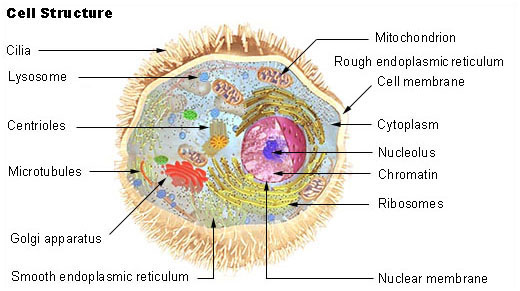
\includegraphics[width=0.8\textwidth]{bilder/Illu_cell_structure.jpg}
\caption{En eukaryot cells anatomi. Cytoplasman innehåller många olika organeller av varierande storlek. \footnotesize Bilden är allmän egendom\cite{wiki:illu_cell_structure} (en: public domain) och får därför reproduceras fritt.}
\label{fig:cell_struktur}
\end{figure}

%By OpenStax College [CC BY 3.0 (http://creativecommons.org/licenses/by/3.0)], via Wikimedia Commons

\subsection{Transport inom cellen}

Att partiklar, från små näringsämnen till stora proteiner, kan ta sig fram genom cytoplasman spelar onekligen en viktig roll för många funktioner i cellen. Om exempelvis näringen vi stoppade i oss inte skulle nå cellernas energifabriker, mitokondrierna, tillräckligt snabbt eller komma fram i för liten skara skulle kroppen med stor sannolikhet snabbt upphöra att fungera. Detta då många av cellens funktioner är starkt beroende av det ATP som mitokondrierna\footnotemark{} producerar.
\footnotetext{Även om en mindre mängd ATP kan produceras även utan mitokondriernas hjälp bildas majoriteten av ATP:n just här \cite{Solunetti_ATP}.}

I celler talar definieras två typer av transport i cytoplasman: den aktiva och den passiva transporten. Under den aktiva transporten vandrar motorprotein längs med proteintrådar och för med sig det som ska transporteras. Under den passiva transporten tillåts ämnena diffundera fritt genom cytoplasman, vilket tillskillnad från driften av motorproteinerna inte kräver energi. 
Vilket transportsystem som är dominerande beror på vilken celltyp som betraktas. I mer primitiva celltyper så som bakterier och jästceller dominerar den passiva transporten medan det i celltyper som bildar stora avancerade och sammanhängande organismer, till exempel djur och växtceller, är vanligare med en dominant aktiv transport. 
%\todo{Varför?} För att tillgodose det ökade behovet av ordning och snabb transport?

Förutom aktinfilamenten som beskrivs i avsnittet nedan finns i cellen även lite tjockare proteintrådar kallade mikrotubuli. Dessa är inte symmetriska utan har en orientering där deras ena ände kallas ''$+$'' och den andra ''$-$''. Längs dessa proteintrådar kan så kallade motorprotein vandra samtidigt som de på sin ovansida fäster tag i något annat för att transportera detta längs med strängen. Det finns en typ av motorprotein som går från ''$+$'' till ''$-$'' och en annan typ som går åt motsatt håll. Då dessa mikrotubuli oftast sitter ordnade i grupp med samma sida inåt möjliggörs den aktiva transporten inom cellerna genom att rätt sorts motorprotein tillåts binda till det som behöver transporteras in mot cellens mitt eller ut mot cellens ytterkanter. 

%Förutom att transportera organeller och membranförslutna paket kan strukturen med dessa tjockare proteintrådar med rätt sorts motorproteiner även hålla vissa membranomslutna organeller på plats. Till exempel skulle Golgiapparaten, som är med och ser till att de syntiserade proteinerna i cellen hamnar på rätt plats, splittras upp i bitar och spridas runt i cellen om den inte hölls på plats mot cellens mitt av inåtvandrande motorproteiner. Även vid anafasen, som är en av faserna under celldelning där de duplicerade kromosomerna separeras så att de två sidorna av cellen får var sin kompletta uppsättning av dem, spelar mikrotubuli och motorproteiner en viktig roll.

Alla dessa proteintrådar skulle kunna påverka cytoplasmans genomtränglighet och i nuläget råder viss oenighet gällande hur cytoplasman egentligen ter sig för partiklar som rör sig genom den. Man har länge trott att cytoplasman upplevs olika beroende på partiklarnas storlek. Små partiklar upplever en kolloid vätskefas där de är väl blandade i cytoplasman medan större partiklar, på grund av sin storlek, ser cytoplasman som ett sammanhängande nätverk av interagerande komponenter. Det senare ger cytoplasman ett mer fast eller glasliknande tillstånd. Nya rön~\cite{Parry_etal2014} spekulerar dock i att dessa upplevda faser hos cytoplasman kan regleras och ändra karaktär.

Det finns även vissa teorier om att partikelrörelsen i celler skulle kunna påverkas av den sammanlagda effekten av motorproteinernas framryckningar. Även om dessa på liten skala ter sig väl riktade och ordnade kan den sammanlagda effekten av alla dessa transporter resultera i en stokastisk kraft som därmed påverkar partikelns rörelsemönster. 

\todo[color=lime]{Ska man nämna exempel?}Passiv transport i celler delas in i fyra processer: diffusion, underlättad diffusion, osmos och filtrering~\cite{Cram_Passivetransport}. Diffusion omfattar netto transport av partiklar från områden av högre koncentration till områden med lägre koncentration. Underlättad diffusion sker för större partiklar som av sig själva inte kan diffundera genom cellmembran. Transportproteiner i cellmembranet möjliggör dock denna transport som kan ske utan energitillförsel, dvs med koncentrationsgradienten. Diffusion av vatten genom membran anses vara en tillräckligt viktig process för att få ett eget namn; osmos. Filtrering sker för partiklar och vatten genom porer i membranet med hjälp av blodtrycket.\todo[color=lime]{Här ska fixas lite}


\subsection{Cellens olika faser}

Under odling av celler kommer kolonin genomgå tre distinkta faser~\cite{Heidcamp_Cellfas}. Initialt, under \emph{lag-fasen}, anpassar sig cellerna till omgivningen under vilket få nya celler produceras. Denna fas varar som mest någon dag och följs sedan av \emph{log-fasen} där celltillväxten sker exponentiellt. Denna fas består tills något näringsämne begränsar tillväxten. Om näring tillförs kontinuerligt till kolonin avstannar tillväxten och cellantalet når en platå, \emph{stationärfas}. Denna fas kan även nås om utrymmet tillgängligt för kolonin är begränsat då tätt-packade celler inte delar sig. 
Om näring inte tillförs kommer istället cellantalet att minska och kolonin kommer in i \emph{dödsfasen}.

Utöver dessa faser kan vissa cell-typer gå i dvala, en överlevnadsfas får tider då näringen är bristfällig eller klimatet ogynnsamt. Om man till exempel kyler ner jästceller kommer de att stänga ner icke-vitala processer för att dra ner på sin ämnesomsättning och därmed gå i dvala. \todo[color=lime]{Här ska vettig källa infogas} 
%http://bakingbabies.se/tag/jast-i-dvala/ %Torrjäst
%https://pilsnerbryggeriet.wordpress.com/tag/jast/


\section{Aktinfilament}

Aktinfilament, även kallat F-aktin, skapas genom att fria G-aktin binds till varandra och bildar polymerer. Denna process kan ske spontant i en aktinlösning och går då åt båda hållen så att filament både byggs upp och bryts ner. Utifrån en kort filamentbit kan därmed en längre kedja byggas upp men på grund av att G-aktinet inte är helt symmetriskt utan har en orientering kommer tillväxten att ske snabbare i ena änden än den andra. Asymmetrin för de enskilda monomererna gör att hela filamentet i sig får en orientering vilket bland annat möjliggör dess användning som transportväg för motorproteiner. Denna syntes av aktinfilament sker cirka 100 gånger snabbare inuti celler än utanför celler i laboratorium då cellen har hjälp av en mängd  katalyserande proteiner med både uppbyggande och nedbrytande egenskaper. Dessa proteiners aktivitet kan i sig regleras och fås att öka eller minska som respons på visst stimuli.

Varje G-aktin i filamenten sitter lite vridet i förhållande till sina grannar vilket leder till att filamenten får formen av en dubbelhelix med bredd på ca 7\,nm och upp till flera mikrometer långa. Dessa dubbelhelixar kan i sin tur kopplas samman av andra proteiner till mer avancerade 3-dimensionella strukturer.
\todo{källa}

Större delen av aktinfilamenten finns koncentrerade strax innanför cellmembranet där de kopplats ihop till ett nätverk som både ger cellen form och stadga samtidigt som det möjliggör transport. Detta nätverk har egenskaper liknande de som återfinns hos semisolida geler. Förutom att bilda 3-dimensionella nät kan aktinfilamenten även ordnas parallellt i mer tätpackade buntar. De buntar som ligger tätast packade ger stöd åt utstickande strukturer från cellmembranet, exempelvis microvilli. De lite mer löst packade används tillsammans med motorprotein i strukturer som har förmågan att kontrahera, något som möjliggör sista steget i celldelningen där själva cellen delas i två. 
%Ett annat exempel är kroppens alla muskler som består av strukturer av aktintrådar och motorproteinet myosin.
\todo{källa}

%Som ett sista exempel kan nämnas att aktinfilament fyller en viktig funktion när cellen i sig förflyttar sig i sin omgivning. Cellen ändrar då form genom att skjuta fram ett utskott framför sig, fäster tag och drar sig fram en bit för att sedan upprepa processen.


\section{Jästceller}
%Datan som detta arbete bygger på kommer från observationer av partikelrörelse i jästceller, så här följer en kort introduktion till jäst. 

Jäst hör till riket svampar och utgörs av encelliga organismer~\cite{SGD_yeast}.
De finns att finna på växter, i jorden men även på huden och i tarmkanalen hos varmblodiga djur. 
%Jästen kan där leva antingen i symbios med värddjuret eller som parasit och i värsta fall orsaka värddjuret skada. 
Att jästen är en encellig organism möjliggör snabb reproduktion vilket gör den smidig att arbeta med i laboratorium. Dessutom uppvisar de större likhet med djurceller än de likväl encelliga bakterierna och ger därmed ges större möjlighet till att dra paralleller till djurceller med försök på jästceller. 

\subsection{Jästcellers cytoplasma}
Att jästceller är svampar innebär att de därmed varken är djur, växter eller bakterier men delar vissa likheter med alla tre celltyper. Med sitt arvsanlag samlat i en cellkärna~\cite{SGD_yeast}, precis som djur- och växtceller, skiljer sig jästceller från bakterier där arvsanlaget ligger blandat med resten av beståndsdelarna i cytoplasman.
De har även en vakuol och stabiliserande cellvägg som växtceller men saknar växtcellens kloroplaster och kan därmed inte utföra någon fotosyntes. Att jästcellen har en cellvägg innebär att den inte är lika beroende av ett stabiliserande proteinfilamentsnätverk och därmed endast har ett rudimentärt sådant~\cite{Midtveldt_etal2016}.

\subsection{Jästcellers transport inom cellen}
Djurcellernas komplicerade nät av proteintrådar, som möjliggör en aktiv transport inom cellen,, finns inte hos jästceller~\cite{Midtveldt_etal2016} som istället får förlita sig på passiv transport, förutom vid celldelning. 
Med jästceller kan man därför undersöka om anomalier från brownsk rörelse, som beskrivs i kommande kapitel, uppkommer även utan de stokastiska krafter med ursprung i det kollektiva bidraget från motorproteinernas framryckningar.


\section{Cellers metabola tillstånds påverkan på partikelrörelsen}
Tidigare studier~\cite{Gou_etal2014} på eukaryota celler har visat att
partiklars rörlighet i cytoplasman beror på hur aktiv cellen
är. Rörligheten för de i dessa studier undersökta cellerna ökade exempelvis
trefaldigt om cellen drabbats av cancer jämfört med en normalt
fungerande cell. En cell som drabbats av cancer kommer att ha en förhöjd metabolism\cite{Gou_etal2014} för att öka på celldelningstakten och kanske är det i samband med detta som även diffusionen i cytoplasman ökar. En möjlig förklaring till fenomenet utpekas i dessa studier som icke-termiska fluktuationer orsakade av motorproteinernas sammanlagda aktivitet.

Studier~\cite{Parry_etal2014} på bakterier har samtidigt visat att
partiklarnas rörlighet minskade drastiskt om den metabola aktiviteten
minskade. Då bakterier saknar aktiv transport i sina celler försökte man här istället nå en förklaring där cytoplasman blir mer vätskelik ju högre aktiviteten är och börjar
likna ett mer elastiskt fast material då aktiviteten
minskar. Partikelstorleken tycks också vara en faktor för dess förmåga
att röra sig runt i cellen. I gränsen när partiklarna närmar sig
storleken av organellerna i cytoplasman blir förklaringen uppenbar;
partikeln kommer då på grund av sin storlek inte att kunna röra sig
runt i cellen som vid fri diffusion. 

Jästceller har förmågan att kunna gå i dvala, ett tillstånd där de
intracellulära aktiviteterna minskar. Då delar av den tillhandahållna
datan kommer från celler i dvala möjliggör detta undersökningar om
huruvida cytoplasmans beståndsdelars rörlighet i cellen även i detta arbete kan bekräftas bero på
cellens metabola tillstånd. 

%Bara en liten kodsnutt som behövs när man kompilerar lokalt
%%% Local Variables: 
%%% mode: latex
%%% TeX-master: "00main.tex"
%%% End: 



%\part{Huvuddel}

\chapter{Stokastiska processer och differentialekvationer}

%För att beskriva de system som undersöks i den här studien behövs stokastisk analys. 
Många fysikaliska system kan beskrivas med ordinära eller partiella differential\-ekvationer (ODE:er
eller PDE:er). Tillräckligt små objekt kommer dock att påverkas betydligt av termiska fluktuationer. Dessa fluktuationer kan betraktas som helt slumpmässiga, varför de då bör beskrivas med \emph{stokastiska processer}. Påverkan på ett system från en stokastisk process leder till att den styrande differentialekvationen behöver modifieras med exempelvis en stokastisk term; det blir då en \emph{stokastisk differentialekvation} (SDE).  Således introducerar följande avsnitt några viktiga begrepp och metoder som används för att studera rörelsen av partiklar i celler samt strängar i vätskor. 

Ett exempel på ett system som består av så ''små objekt'' att termiska
fluktuationer behöver beaktas är i så kallad \emph{brownsk rörelse}. 
Detta är ett fenomen där små partiklar vandrar runt slumpmässigt, till synes av sig själva. Fenomenet beskrevs först av Robert Brown som 1827~\cite{Brown1828} upptäckte att partiklar från pollenkorn rörde sig hackigt när de flöt på vatten. Fenomenet förklarades dock först 1905 av Einstein \cite{Einstein1905}. Förklaringen går ut på att partiklarna är små nog för att kollisioner med vattenmolekyler ska överföra tillräckligt med rörelsemängd för att pollenkornens rörelseändringar ska bli synbara i ett mikroskop. 


\section{Stokastiska processer}
En \emph{stokastisk variabel} $X$ är ett objekt som kan anta värden
$x$ från en viss värdemängd $\Omega$. Vilka värden som antas styrs av
sannolikhetsfördelningen $p(x)=P(X=x)$. I fallet med diskreta stokastiska
variabler är sannolikhetsfördelningen helt enkelt sannolikheten att
$X$ antar värdet $x$. Men i det här arbetet ligger fokus på
kontinuerliga stokastiska variabler. För dessa gäller att sannolikheten för att $X$ antar ett värde i intervallet $[x, x+\dd{x}]$ ges av
\begin{equation}
P\big( X\in[x, x+\dd{x}] \big) =p(x)\dd{x}
\end{equation}
för någon infinitesimal intervallbredd $\dd{x}$ och där $p(x)$ är sannolikhetstätheten av $X$ i $x$. 
I fortsättningen av detta arbete kommer ''stokastisk variabel'' att avse en \emph{kontinuerlig} stokastisk variabel om inget annat anges.


Från detta kan en så kallad \emph{stokastisk process} definieras som en samling av objekt som beror på en stokastisk variabel $X$ och en deterministisk variabel, ofta betraktad som en tid\footnotemark{} $t$.
I denna rapport studeras stokastiska processer $Y(t)$ som är funktioner $Y(t) = f(X,t)$, där $X$ följer sannolikhetsfördelningen $p(x)$. Processen $Y(t)$ beror alltså implicit på den stokastiska variabeln $X$.
\footnotetext{Att tiden väljs som deterministisk variabel är anledning till att det kallas stokastisk \emph{process}. Tanken är att ett tidsförlopp som beror av den stokastiska variabeln utspelar sig. Mer generellt kan en godtycklig deterministisk variabel användas istället för tid.}  

\subsection{Statistiska verktyg för att undersöka stokastiska processer}
Stokastiska processer är som sagt slumpartade processer. Därmed kan det vara svårt att avgöra processens natur enbart utifrån ett fåtal observationer. För att kunna undersöka en stokastisk process behövs olika statistiska verktyg som exempelvis väntevärde och korrelation.

\subsubsection{Väntevärde, varians och kovarians}
För en stokastisk variabel $X$ definieras \emph{väntevärdet} med hjälp av variabelns sannolikhetsfördelning $p(x)$ enligt
\begin{equation}\label{eq:EV}
    \ev{X} = \int_{\Omega} x p(x) \id{x}.
\end{equation}
Något löst sett kan detta betraktas som det förväntade medelvärdet vid upprepade mätningar av $X$. En av de viktigaste egenskaperna hos väntevärdet är att det är \emph{linjärt}. Alltså att~\cite{Rice_matstat2006}
\begin{equation}\label{eq:EV_linkomb}
\ev{a+\sum_{i=1}^N b_i X_i} = a+\sum_{i=1}^N b_i \ev{X_i}
\end{equation}
för konstanterna $a$ och $b_i$ samt stokastiska variablerna $X_i$. 

Väntevärdet går även att utvidga till att även omfatta funktioner av
den stokastiska variabeln. Vilket ges av~\cite{Rice_matstat2006}
\begin{equation}\label{eq:EV_f}
    \ev{f(X)} = \int_{\Omega} f(x) p(x) \id{x}.
\end{equation}
Speciellt i fallet med stokastiska processer blir väntevärdet 
\begin{equation}\label{eq:EV_process}
    \ev{Y(t)} = \int_{\Omega} Y(t)p(x) \id{x},
\end{equation}
notera att väntevärdet är beroende av $t$. Läsaren påminns om att $Y(t)$ implicit beror av $X$.

Vidare definieras det $n$:te momentet enligt 
\begin{equation}
\Big\langle Y(t_1)Y(t_2)..Y(t_n) \Big\rangle 
= \int_{\Omega} Y(t_1)Y(t_2)\ldots Y(t_n)p(x)\id{x}.
\end{equation}
Om momentfunktionen är oberoende av en translation i tid $t_i\to t_i+\tau$, där $i=1,2,\ldots,n$, för alla val av $n$ och $t_i$ definieras den stokastiska processen som \emph{stationär}. Speciellt är väntevärdet $\ev{Y(t)}$ oberoende av $t$ för en stationär process. 

Om väntevärdet är ett mått som anger vad man förväntas få som medelvärde, så behövs även ett mått på hur spridda värden man kan tänkas få. För det används \emph{variansen}, som går att formulera på några olika sätt~\cite{Rice_matstat2006}
\begin{equation}\label{eq:VAR}
\sigma_X^2=\VAR{X} = \ev{\big(X-\ev{X} \big)^2} = \ev{X^2}-\ev{X}^2.
\end{equation}
Dock ger variansen, som man kan se, ett kvadratiskt mått på avvikelser från medelvärdet. Därför kan det, exempelvis i sammanhang där man vill jämföra spridningen i en mätserie, vara mer intressant att betrakta \emph{standardavvikelsen} $\sigma_X$ som ges av roten ur variansen.


På ett analogt sätt definieras en \emph{kovarians}~\cite{Rice_matstat2006}
\begin{equation}\label{eq:COV}
\COV{X}{Z} 
= \Big\langle \big(\, X-\ev{X}\big) \big(\, Z-\ev{Z}\big) \Big\rangle
= \ev{XZ}-\ev{X}\ev{Z}.
\end{equation}
Kovariansen är ett mått på hur mycket två stokastiska variabler samvarierar. Speciellt syns också att $\COV{X}{X}=\VAR{X}$; alltså att kovariansen övergår i variansen för $Z=X$. Vidare gäller att om variablerna är \emph{statistiskt oberoende} så är kovariansen 0.

För att beräkna variansen av en linjärkombination av stokastiska variabler utnyttjas \eqref{eq:EV_linkomb} tillsammans med definitionerna av varians och kovarians. Då erhålls
\begin{equation}
\VAR{a+\sum_{i=1}^N b_i X_i} = \VAR{\sum_{i=1}^N b_i X_i} 
= \sum_{i=1}^N\sum_{j=1}^N b_i b_j\, \COV{X_i}{X_j}.
\end{equation}
Om $X_i$ är oberoende, så att $\COV{X_i}{X_j}=0$ för $i\neq j$, kan det sista ledet skrivas om till
\begin{equation}\label{eq:VAR_linkomb}
\VAR{a+\sum_{i=1}^N b_i X_i} = \sum_{i=1}^N b_i^2\, \VAR{X_i}.
\end{equation}




\subsubsection{Korrelationsfunktioner}
I fallet med stokastiska processer kan det även vara intressant att veta hur korrelerade två processer $Y_1(t)$ och $Y_2(t)$ är, i till exempel tiden. För det används \emph{korrelationsfunktionen}
\begin{equation}\label{eq:corr}
\kappa_{12}(t, t') = \ev{Y_1(t)Y_2(t')}.
\end{equation}
Oftast brukar också de undersökta processerna ha väntevärde $0$; då övergår $\kappa_{12}$ till att bli kovariansen mellan $Y_1(t)$ och $Y_2(t')$, vilket underlättar tolkningen att $\kappa_{12}$ svarar mot en sorts korrelation. 

Ett specialfall som ofta används är den så kallade \emph{autokorrelationsfunktionen} 
\begin{equation}\label{eq:autocorr}
\kappa_{YY}(t, t') = \ev{Y(t)Y(t')}.
\end{equation}
Som helt enkelt är när samma process undersöks i olika tidpunkter. 

Om de stokastiska processerna är stationära, vilket ofta gäller, innehar korrelationsfunktionen translationssymmetri i $t$, alltså att när man väljer sitt origo inte spelar någon roll. Detta gör att $t$ och $t'$ kan ersättas differensen~$\tau=\Delta t= \abs{t-t'}$:
\begin{equation}
\kappa_{12}(\tau) = \kappa_{12}(t, t+\tau).
\end{equation}
%Detta är en egenskap som kommer utnyttjas flitigt under resten av den här studien.

Här bör också påpekas att en \emph{normerad} korrelationsfunktion ibland används men ändå bara kallas ''korrelationsfunktion''. Det kännetecknande för de normerade korrelationsfunktionerna är att de bara antar värden mellan $-1$ och $1$.


\subsubsection{Kovariansmatris}\label{sec:kovmatris}
För att studera kovariansen mellan flera stokastiska processer $Y_i(t)$, där $i=1,2,\ldots,n$ och $n$ är antalet processer, kan en kovariansmatris definieras. Där svarar varje element mot kovariansen mellan process $i$ och process $j$. I denna studie används en tidsoberoende kovariansmatris definierad enligt 
\begin{equation}
\label{eq:kovmatris}
    \mathsfit{C}_{ij} = \COV{Y_i(t)}{Y_j(t)}_t
\end{equation}
där kovariansen är bildad med avseende på tiden. Om kovariansmatrisen är icke-diagonal är de stokastiska processerna korrelerade. Kovariansmatrisen ses enligt denna definition vara symmetrisk samt reell, givet att $Y_i(t)$ är reella stokastiska processer. Således är den även diagonaliserbar, och enligt spektralsatsen är dess egenvärden reella. 

Diagonalisering av kovariansmatrisen åstadkoms genom ett basbyte till en bas bestående av linjärkombinationer av de stokastiska processerna, dessa linjärkombinationer är okorrelerade~\cite{Shlens_PCA2014} och är egenvektorer till $\mathsfit{C}$. Egenvärdena till kovariansmatrisen svarar mot variansen av motsvarande egenvektor.


\subsection{Skattningar med diskret data} \label{sec:diskret_data}
Alla verktygen ovan bygger på olika väntevärden. Så för att kunna tillämpa dessa statistiska metoder behövs ett stort statistiskt underlag, baserat på många observationer. Med detta statistiska underlag kan sedan skattningar av exempelvis väntevärde och varians göras.

Vid statistiska analyser används alltså medelvärdet i en mätserie för att approximera väntevärden. Så skattningen ges av
\begin{equation}\label{eq:mean}
\ev{X} \approx \bar{x} = \frac{1}{N} \sum_{i=1}^N x_i,
\end{equation}
där $x_i$ är de olika observationerna av $X$ och $N$ dess totala antal. 

När man ska beräkna variansen från ett stickprov kräver båda uttrycken i \eqref{eq:VAR} två väntevärden. Om inte $\ev{X}$ är känt får man alltså in två approximationer när man använder \eqref{eq:mean} för att beräkna väntevärdena i \eqref{eq:VAR}. Detta bidrar bland annat till att en approximation av standardavvikelsen behöver göras enligt
\begin{equation}\label{eq:standard_error}
\sigma_X^2 \approx s_X^2
=  \frac{1}{N-1} \sum_{i=1}^N \left(x_i-\bar{x}\right)^2.
\end{equation}
Detta är standardfelet, $s_X$, i kvadrat beräknat med Bessels korrektion, som innebär att man använder $N-1$~\cite{Rice_matstat2006} i nämnaren istället för bara $N$. Approximationen av kovariansen följer helt analogt från \eqref{eq:COV}.

\subsubsection{Noggrannheten av skattningarna}
För att dessa skattningar ska kunna användas behöver man veta hur bra de är. I bilaga~\ref{sec:noggrannhet} bevisas att både \eqref{eq:mean} och \eqref{eq:standard_error} är obiaserade i väntevärdesmening. Alltså att väntevärdet av skattningarna faktiskt är den storhet som skattas.

Vidare behövs även hur stor standardavvikelse man förväntas få i skattningarna. Denna noggrannhet beräknas i bilaga~\ref{sec:noggrannhet}. I huvudsak kan man säga att felet i en skattning av väntevärdet eller varians\footnotemark{} minskar ungefär som $1/\sqrt{N}$ i båda fallen -- ska man däremot skatta en populations standardavvikelse blir felet roten av detta. 
Detta betyder att man i princip kan komma godtyckligt nära det verkliga värdet genom att öka antalet mätvärden.
\footnotetext{I beräkningarna av osäkerheteten i skattningen av variansen användes att $N$ behövde vara stort. För osäkerheten i skattningen av väntevärde behövs dock ingen sådant antagande. }

%\subsection{Normalfördelnigen}


\subsection{Spektral effekttäthet (PSD)} \label{sec:PSD}

Inom bland annat signalbehandling kan det vara intressant att veta vilka frekvenskomponenter en signal innehåller. Generellt sett används fouriertransformen för att ta fram en signals spektrum.
För stokastiska processer kan liknande metoder användas, men tyvärr är i allmänhet stokastiska processer inte fouriertransformerbara. Istället används den så kallade spektrala effekttätheten, även kallad PSD (en. power spectral density), en nära släkting till fouriertransformen.

%\paragraph{Energi- och effektinnehåll i en stokastisk process}
Energin i en process $Y(t)$ kan betraktas som integralen
\begin{equation}\label{eq:energy}
E_Y(T) = \int_{-T}^{T} \abs{Y(t)}^2\id{t},
\end{equation}
där $T$ svarar mot den tid som energin mäts över. Anledningen till att stokastiska processer i allmänhet inte är fouriertransformerbar är att denna integral divergerar när $T\to\infty$. Alltså att $Y$ är divergent i $\mathcal{L}^2$-mening. 

För att få kopplingen att \eqref{eq:energy} svarar mot just \emph{energin} i processen kan $Y(t)$ betraktas som en spänning, vilket ger att $\abs{Y(t)}^2$ är proportionellt mot effekten; integreras sedan en effekt över tid så erhålls en energi. I övriga fall väljer man oftast att kalla motsvarande storheter för energi och effekt trots att de kanske inte strikt sett går att betrakta dem som fysikaliska energier eller effekter. 

För att undvika divergens när $T\to\infty$ betraktas istället medeleffekten 
\begin{equation}\label{eq:power}
P_Y(T) = \frac{1}{2T} \int_{-T}^{T} \abs{Y(t)}^2\id{t},
\end{equation}
som för de flesta stokastiska processer oftast~\cite{Miller_probability2012} beter sig bättre än energin.
I det här läget är det också viktigt att påpeka att trots att $P_Y$ kallas medeleffekt, så är det bara medeleffekten av ett visst utfall av den stokastiska processen $Y$, och bör \emph{inte} förväxlas med någon form av väntevärde. 

För att till slut koppla samman detta med spektraltätheter används den spektrala effekttätheten eller PSD:n
\begin{equation}\label{eq:PSD}
\mathcal{S}(f) =  \lim_{T\to\infty}\dfrac{1}{2T} \ev{\abs{\hat{Y}_T(f)}^2},
\end{equation} 
där
\begin{equation}\label{eq:truncated_F}
\hat{Y}_T(f) = \int_{-T}^{T} Y(t)\,\ee^{-\ii 2\pi f t} \id{t}
\end{equation}
är den trunkerade fouriertransformen av $Y$. Genom att ta med kvoten $\nicefrac{1}{2T}$ i \eqref{eq:PSD} erhålls en spektraltäthet av effekter som kan konvergera även om \eqref{eq:truncated_F} på egen hand divergerar när $T\to\infty$. 

\subsubsection{Wiener-Khinthchine-teoremet}
För att sen koppla ihop PSD:n med några av processens reella egenskaper används Wiener-Khinthchine-teoremet. Kortfattat så säger det att för stationära processer som är ''tillräckligt snälla'' är \cite{Miller_probability2012}
\begin{equation}\label{eq:W-K-theorem}
\mathcal{S}(f) = \mathcal{F}\left[\kappa_{YY}(\tau)\right] 
= \int_{-\infty}^{\infty} 
\kappa_{YY}(\tau) \ee^{-\ii 2\pi f\tau} \id\tau,
\end{equation}
alltså att PSD:n och autokorrelationsfunktionen är kopplade genom fouriertransform. 

Vad som menas med ''tillräckligt snälla'' processer framgår om man tittar på resonemanget som leder fram till beviset av \eqref{eq:W-K-theorem}. Det börjar med att betrakta högerledet i \eqref{eq:PSD}
\begin{equation}
\begin{aligned}
\ev{\abs{\hat{Y}_T(f)}^2}&=\ev{\hat{Y}_T(f)\,\hat{Y}_T^*(f)}\\
&=\ev{
\int_{-T}^T\int_{-T}^T\!\dd{t}\dd{t'} Y(t)\ee^{-\ii 2\pi ft}
 \;Y(t')\ee^{+\ii 2\pi ft'}
}\\
&=\int_{-T}^T\int_{-T}^T\!\dd{t}\dd{t'} 
\ev{Y(t)Y(t')} \ee^{-\ii 2\pi f(t-t')}.
\end{aligned}
\end{equation}
Efter det här steget utnyttjas definitionen av $\kappa$ i \eqref{eq:autocorr} och att $Y$ är stationär, så att
\begin{equation}
\ev{Y(t)Y(t')} = \kappa_{YY}(t, t') = \kappa_{YY}(t-t').
\end{equation}
Härifrån noteras att $(t-t')$ även förekommer i exponenten så transformen ser ut att kunna gå ihop. Därefter används lite finurliga variabelsubstitutioner och geometriska resonemang~\cite{Miller_probability2012} för att slutligen landa i \eqref{eq:W-K-theorem}.

En tillräckligt snäll process är alltså en process som tillåter att väntevärdet flyttas in under integraltecknen. Detta är oftast inga problem i de flesta fysikaliska tillämpningar. 


\subsection{Vitt brus och Wienerprocessen}\label{sec:white_noise}
Vitt brus, $\pd_tW(t)$,\footnotemark{} är ett brus med konstant PSD, det har alltså lika mycket av alla frekvenskomponenter. Det går att visa att vitt brus uppfyller \cite{Miller_probability2012}
\begin{equation}\label{eq:white_noise}
\begin{aligned}
\ev{\pd_tW(t)}&=0 \\
\ev{\pd_tW(t)\pd_{t'}W(t')}&=  \delta(t-t'),
\end{aligned}
\end{equation}
samt är normalfördelat. 
Det bör nämnas att äkta vitt brus inte är fysikaliskt eftersom det innehåller oändligt mycket energi. I de flesta tillämpningar brukar dock fluktuationer antas vara vitt brus för att det oftast ger enkla teoretiska analyser. Vidare kan även verkligt brus i många fall~\cite{Engelberg_noise2007} betraktas som vitt till en god approximation -- det vill säga har en konstant spektralfördelning i ett begränsat frekvensintervall. 
\footnotetext{Beteckningen med en tidsderivata $\pd_t$ kan verka märklig, men det kommer från tolkningen av Wienerprocessen som integralen av vitt brus. Det står mer om detta längre ner i det här avsnittet.}

Att \eqref{eq:white_noise} medför konstant PSD inses genom att betrakta
\begin{equation}
    \ev{\abs{\widehat{\pd_tW}_\omega(f)}^2} =
    \int_{-T}^{T}\int_{-T}^{T}\!\dd{t}\dd{t'}
    \ev{\pd_tW(t)\pd_{t'}W(t')}\ee^{-i2\pi f(t-t')},
\end{equation}
som är den trunkerade fouriertransformen \eqref{eq:truncated_F} av $\pd_tW(t)$. Denna integral kan beräknas med hjälp av \eqref{eq:white_noise}
\begin{equation}
    \int_{-T}^{T}\int_{-T}^{T}\!\dd{t}\dd{t'} 
     \delta(t-t')\ee^{-i2\pi f(t-t')} 
    =  \int_{-T}^{T}\dd{t} =2T.
\end{equation}

Således ses att \eqref{eq:white_noise} medför 
\begin{equation} \label{eq:white-noise_PSD}
    \mathcal{S}(f) = \lim_{T\to\infty}\dfrac{2T}{2T} = 1,
\end{equation}
vilket visar att PSD:n är konstant. 


%Strikt talat ges en Wienerprocess genom att börja med att betrakta \cite{Miller_probability2012}
%\begin{equation}
%\tilde{W}(t) = \sum_{k=1}^{n} \delta X_i,
%\end{equation}
%där $X_i$ är oberoende stokastiska ''steg'' med som enbart kan anta värdena $1$ och $-1$ med $P(X=1)=P(X=-1)=\nicefrac{1}{2}$, och där $n=t/\Delta{t}$ är antalet steg som tas. Genom att låta $\Delta{t}$ och $\delta$ samtidigt gå mot 0 erhålls en äkta Wienerprocess. 

En Wienerprocess $W(t)$ är en tidskontinuerlig stokastisk process som kan betraktas som integralen av vitt brus\cite{Miller_probability2012}. Detta är anledningen till att det vita bruset har betecknats som tidsderivatan av en Wienerprocess: $\pd_tW(t)$. Vidare brukar integraltolkningen leda till att Wienerprocessen beskrivs som den matematiska beskrivningen av brownsk rörelse. 

Ur en praktisk synvinkel är det dock lättare att tänka sig Wienerprocessen som summa av ett antal normalfördelade steg. Betrakta summan
\begin{equation}\label{eq:wiener_approx}
\tilde{W}_n = \sum_{k=1}^{n} \epsilon X_i,
\end{equation}
där varje steg $X_i$ är normalfördelat $N(0,1)$ och $n$ är antalet steg. 
Wienerprocessen erhålls sedan i gränsen där $n\to\infty$ och $\epsilon\to 0$ samtidigt\cite{Miller_probability2012}. Detta åskådliggör tolkningen av Wienerprocesssen som integralen av vitt brus eftersom summan i viss mån kan tolkas som en Riemannsumma som övergår till en integral i den gränsen.

Från \eqref{eq:wiener_approx} erhålls att 
\begin{equation}
\ev{\tilde{W}_n} = \epsilon\sum_{i=i}^n \ev{X_i} = 0
\end{equation}
och
\begin{equation}
\VAR{\tilde{W}_n} = \epsilon^2 \sum_{i=i}^n \VAR{X_i} = n\epsilon^2.
\end{equation}
Genom att betrakta \eqref{eq:wiener_approx} som en approximation för Wienerprocessen, är det troligt att den riktiga Wienerprocessen har liknande egenskaper. Så visar sig också vara fallet~\cite{Miller_probability2012}
\begin{equation}
\begin{aligned}
\ev{W(t)} &= 0\\
\VAR{ W(t) } = \ev{ (W(t))^2 } &\propto t.
\end{aligned}
\end{equation}
Dess egenskaper utnyttjas i avsnitt~\ref{sec:brown} om brownsk rörelse.



%Tror det blir onödigt formellt att matematiskt definiera dessa

%\subsection{Integraler med stokastiska integrationsvariabler}
%\label{sec:Stok_int}

%Integraler med stokastiska intebrationsvaribler skiljer sig från integraler i den reella analysen då de ofta behandlar icke-deriverbara processer. Därav behövs en ny definition av hur en sådan stokastisk integral ska beräknas. Följande avsnitt här till stor del hämtat från \emph{Brownian motion and stochastic calculus} av I. Karatzas och S. E. Shreve \cite{Karatzas_stokint1991}, t ex.

%\cite{Dieker_fBm} har bra enklare info.








\section{Stokastiska differentialekvationer}
En differentialekvation som innehåller termer bestående av stokastiska processer kallas en stokastisk differentialekvation (SDE). Lösningen till en SDE kommer representeras av en stokastisk process eftersom minst en av de ingående termerna är stokastisk. Detta gör att systemets tidsutvecklingen också är stokastisk.

Inom fysiken modelleras ofta system via dess styrande differentialekvation. För att studera system under påverkan av en stokastisk fluktuation, exempelvis brus i en elektrisk krets, kan en stokastisk term som representerar fluktuationen adderas till differentialekvationen. Detta kallas \emph{Langevinformalism} och motsvarande stokastiska differentialekvation kallas systemets \emph{Langevinekvation}. Ett illustrerande exempel av Langevinformalismen är fallet för brownsk rörelse som beskrivs i avsnitt~\ref{sec:brown}.

Ett problem som kan uppstå här är att fluktuationens stokastiska fördelning är okänd. Oftast görs dock antaganden om fluktuationen så som att den består av vitt brus som i avsnitt~\ref{sec:white_noise}. 
Antaganden om fluktuationens väntevärde och korrelation men med en okänd sannolikhetsfördelning leder till att lösningen av Langevinekvationen endast kan beskrivas med motsvarande storheter för systemet. Alltså studeras under dessa antaganden oftast inte lösningen som sådan, utan istället motsvarande väntevärde samt korrelation för lösningen.  

%\subsubsection{Integrering}
%\todo[inline]{Hur och varför flytta in $\ev{\cdot}$ under integral.}





\subsection{Brownsk rörelse}\label{sec:brown}
Ett illustrerande exempel på en SDE är brownsk rörelse. Här utgår man från Newtons andra lag för att ställa upp en Langevinekvation för partikelns hastighet. Man antar att varje kollision med de omgivande molekylerna ger en stokastiskt bidrag till partikelns rörelsemängd, vilket ger en stokastisk kraftterm i Newtons andra lag.

Hastigheten för en partikel som utför ren brownsk rörelse styrs av
Langevinekvationen~\cite{Mazo_Brownian2002} 
\begin{equation} \label{eq:Brownian_SDE}
    M\pd_tv=-\zeta v + F(t),
\end{equation}
där $M$ är partikelmassan, $\zeta$ en friktionskonstant och $F(t)$ den stokastiskt fluktuerande kraften. Kraften utgör här det stokastiska bidraget antas uppfylla egenskaperna för vitt brus enligt \eqref{eq:white_noise}, men med en extra faktor $\sigma$ multiplicerad med korrelationen.
%Den fysikaliska tolkningen av denna stokastiska kraft är att partikeln får små impulser från omgivande vätskepartiklar vilka kolliderar slumpmässigt med partikeln.  


Lösningen till den stokastiska differentialekvationen
\eqref{eq:Brownian_SDE} ges av  
\begin{equation}
v(t)
=v(0)\ee^{-\zeta t/M}
 +\frac{1}{M}\int^t_0 F(\tau)e^{-\zeta (t-\tau)/M} \id\tau.
\end{equation}
Detta får dock inte den stokastiska termen att försvinna och lösningen kan inte skrivas på en deterministisk form. För att ändå kunna göra några förutsägelser betraktas väntevärdet och korrelationen i tiden. Korrelationen ges av, där $\delta t\geq0$,
\begin{equation}\label{Brownian_korr}
\begin{aligned}
\ev{v(t)v(t+\delta t)} 
=& v(0)^2\ee^{-\zeta(2t+\delta t)/M}\\
 &+ \frac{1}{M^2}\ee^{-\zeta (2t+\delta t)/M}
  \int_0^t\int_0^{t+\delta t}\!\dd\tau\dd\tau'\, 
     \ee^{\zeta (\tau+\tau')/M}\ev{F(\tau)F(\tau')}.
\end{aligned}
\end{equation}
Utnyttja att $F(t)$ korrelerar enligt \eqref{eq:white_noise} vilket ger 
\begin{equation} \label{eq:Brown_korr}
\ev{v(t)v(t+\delta t)} 
= v(0)^2\ee^{-\zeta (2t+\delta t)/M}
 +\frac{\sigma^2}{M^2}\ee^{-\zeta (2t+\delta t)/M}
  \int_0^t\!\dd\tau\ee^{2\zeta \tau /M}.
\end{equation}
Korrelationen ovan kan nu enkelt beräknas och genom att låta $\delta t\to 0$ samt $t\to \infty$ fås följande samband
\begin{equation}
    \ev{v(t)^2} = \frac{\sigma^2}{2M\zeta}.
\end{equation}

Med hjälp av detta samband samt ekvipartitionsteoremet som gäller vid termisk jämvikt: $\frac{1}{2}M\ev{v^2}=\frac{1}{2}k_BT$, där $k_B$ är Boltzmanns konstant och $T$ är absoluta temperaturen, kan variansen $\sigma^2$ relateras till fysikaliska storheter enligt
\begin{equation}
    \sigma^2 = 2k_BT\zeta.
\end{equation}
Detta resultat är ett exempel på fluktuation-dissipationsteoremet som relaterar dissipationen av energi, friktionen, med fluktuationen, brownsk rörelse. 

För $t \gg \nicefrac{M}{\zeta}$, det vill säga i gränsen med hög viskositet och lågt Reynoldstal, så kan tröghetstermen i \eqref{eq:Brownian_SDE} försummas relativt friktionskraften. Ekvationen reducerar då till
\begin{equation}
    \zeta \pd_t x=F(t),
\end{equation}
där $x$ är partikelns position. Detta ger lösningen
\begin{equation}
    x(t)=x(0)+\frac{1}{\zeta} \int^t_0 F(\tau)\id\tau.
\end{equation}
Utifrån denna lösning kan medelvärdet av den kvadrerade avvikelsen beräknas, kallat ''mean squared displacement'', MSD, (sv. medelvärdet av det kvadrerade avståndet) vilken blir 
\begin{equation}\label{eq:MSD_brown}
    \ev{(x(t)-x(0))^2}=\frac{2k_BTt}{\zeta} \propto t,
\end{equation}
där enligt fluktuation-dissipationsteoremet  $\sigma^2=2k_BT\zeta$. MSD:n kommer därmed att öka linjärt med tiden, något som enkelt kan jämföras med uppmätt data.




%Bara en liten kodsnutt som behövs när man kompilerar lokalt
%%% Local Variables: 
%%% mode: latex
%%% TeX-master: "00main.tex"
%%% End: 


\chapter{Partikelrörelse i celler}
\todo[inline]{Flytta till cellbiologi. Motivera istället kapitlet.}

%\section{Teori} \todo[inline]{Inga tomma rubriker.}

%\todo[inline]{Fylla ut med lite mera bakgrund/inledning till partikelrörelse.}

%\subsubsection{Metabola tillståndets påverkan på partikelrörelsen}
Tidigare studier~\cite{Gou_etal2014} på eukaryota celler har visat att
partiklars rörlighet i cytoplasman beror på hur aktiv cellen
är. Rörligheten för de i dessa studier undersökta cellerna ökade exempelvis
trefaldigt om cellen drabbats av cancer jämfört med en normalt
fungerande cell. En cell som drabbats av cancer \todo{källa}kommer att ha en
förhöjd metabolism för att öka på celldelningstakten och kanske är det i samband med detta som även diffusionen i cytoplasman ökar. En möjlig förklaring till fenomenet utpekas i dessa studier som icke-termiska fluktuationer orsakade av motorproteinernas sammanlagda aktivitet.

Studier~\cite{Parry_etal2014} på bakterier har samtidigt visat att
partiklarnas rörlighet minskade drastiskt om den metabola aktiviteten
minskade. Då bakterier saknar aktiv transport i sina celler försökte man här istället nå en förklaring där cytoplasman blir mer vätskelik ju högre aktiviteten är och börjar
likna ett mer elastiskt fast material då aktiviteten
minskar. Partikelstorleken tycks också vara en faktor för dess förmåga
att röra sig runt i cellen. I gränsen när partiklarna närmar sig
storleken av organellerna i cytoplasman blir förklaringen uppenbar;
partikeln kommer då på grund av sin storlek inte att kunna röra sig
runt i cellen som vid fri diffusion. 

Jästceller har förmågan att kunna gå i dvala, ett tillstånd där de
intracellulära aktiviteterna minskar. Då delar av den tillhandahållna
datan kommer från celler i dvala möjliggör detta undersökningar om
huruvida cytoplasmans beståndsdelars rörlighet i cellen även i detta arbete kan bekräftas bero på
cellens metabola tillstånd. 


\section{Alternativa modeller för partikelrörelse i vätskor}

Till en första approximation skulle rörelsen för en partikel i en jästcells cytoplasma kunna beskrivas med klassisk brownsk rörelse. Partiklarna krockar där med mindre partiklar från omgivningen och rörelsen kan här beskrivas med en stokastisk gaussisk propagator~\cite{Einstein1905}
\begin{equation}
P(x,t)=\frac{1}{\sqrt{4\pi Dt}}e^{-\nicefrac{x^2}{4Dt}}
\end{equation} %Obs n=1 då endast en partikel följs
som utgörs av sannolikhetsfunktionen för partikelns förflyttning $x$ vid en given tid $t$, där konstanten D är dess diffusionskonstant. Om partikeln betraktas som en sfär med radie $R$ nedsänkt i en vätska med viskositet $\eta$ och absolut temperatur $T$ kan D approximeras till~\cite{Einstein1905}
\begin{equation}
D=\frac{RT}{N}\frac{1}{6\pi \eta R}
\end{equation}
där R är allmänna gaskonstanten och N antalet molekyler som ryms i 1 gram för omgivande fluiden.
\todo{Utveckla mer eller räcker det så här?}
%Man betraktar då cytoplasman som en homogen vätska. %Denna teori bygger dock på att man har termisk jämvikt och att partiklar rör sig i en enbart viskös vätska, två kriterier som inte uppfylls i cytoplasman bland annat på grund av mitokondriernas energiutvinning.

Experiment\cite{Midtveldt_etal2016} har dock visat att diffusionen av partiklar i celler är fundamentalt långsammare än vad man får ut från klassisk brownsk rörelse. Det finns ett par verktyg man kan använda för att undersöka detta. Ett av dem är MSD. Som visades i avsnitt~\ref{sec:brown} är MSD:n för brownsk rörelse proportionell mot förlupen tid. Speciellt kan \eqref{eq:MSD_brown} skrivas om till
\begin{equation}
\ev{x(t)^2} \propto t,
\end{equation}
där $x(0)=0$. Vad man\cite{Midtveldt_etal2016} då har funnit i tidigare studier är att exponenten på $t$ är lägre än $1$, vilket tyder på att andra förklaringsmodeller kan behövas. %Två sådana kandidater är ''Continuous Time Random Walk'' (CTRW) och ''Fractional Brownian motion''.
\todo[inline]{Lägg in fler anledningar varför Brown inte funkar.}

%\subsubsection{Brownsk rörelse} \label{sec:Brownsk}
%\todo[inline]{Skriv ihop kort sammanfattning av det som står i stokastikavsnittet}
%\todo[]{Förklara varför anomal transport ens är intressant att studera.}


\subsection{Ornstein-Uhlenbeck-process}
En första utvidgning av modellen för Brownsk rörelse fås om man lägger till en återförande term som drar partikeln mot någon medelpunkt. Man får då en så kallad Ornstein-Uhlenbeck-process
\begin{equation}\label{eq:SDE_o-u}
\pd_t x = -\gamma ( x-\bar{x} ) + \pd_t W,
\end{equation}
där $\gamma$ är en tidsskala som styr hur hårt bunden partikeln är till medelpositionen $\bar{x}$, och $\pd_t W$ är den stokastiska drivningen av partikeln som uppfyller $\ev{\pd_t W}=0$ och $\ev{\pd_t W(t)\pd_t W(t')} = \sigma^2\delta(t-t')$. Detta är en inte helt orimlig modell eftersom en partikel i en cell rimligtvis inte kan vandra hur långt som helst. Typiskt kommer en partikel att tränga ihop cytoplasmans beståndsdelar i den riktning som den rör sig åt, vilket leder till en återförande kraft.

Med hjälp av \eqref{eq:SDE_o-u} och metoderna från avsnitt~\ref{sec:brown} kan man härleda modellens kovarians och MSD. Kovariansen i gränsen mot ett stationärtillstånd ($\gamma t\gg 1$) blir då
\begin{equation}\label{eq:COV_o-u}
\ev{x(t)x(t+\Delta{t})} \approx \frac{\sigma^2}{2\gamma} \ee^{-\gamma\Delta{t}},
\end{equation}
där $\bar{x}$ har satts till 0. Vidare kan också MSD beräknas till:
\begin{equation}\label{eq:MSD_o-u}
\ev{x(t)^2} 
\approx \frac{\sigma^2}{2\gamma} \left( 1-\ee^{-2\gamma t} \right),
%\approx \frac{\sigma^2}{2\gamma}t\qcomma \text{för } \gamma t\ll1
\end{equation}
med $\bar{x}=0$. Notera att både \eqref{eq:COV_o-u} och \eqref{eq:MSD_o-u} ger att variansen, då $\gamma t\gg 1$, blir konstant lika med~$\nicefrac{\sigma^2}{2\gamma}$ eftersom $\ev{x(t)}=\bar{x}=0$.

%Notera likheten här till den styrande SDE:n för Brownsk rörelse.

%\todo[inline]{Kommer mera så småningom...}
  
\subsection{Continuous Time Random Walk (CTRW)}
En möjlig förklaringsmodell för anomal transport i celler utgörs av CTRW (Continuous-Time Random Walk)~\cite{Hofling&Franosch2013}. Här beskrivs rörelsemönstret av att partiklarna under majoriteten av tiden sitter bundna till olika nätliknande strukturer för att sedan plötsligt ta sig vidare till en ny position efter en viss väntetid. Positionsändringen och väntetiden beskrivs av två oberoende stokastiska variabler. 
MSD för denna typ av rörelse blir\cite{Barkai_CTRW}
\begin{equation}\label{eq:CTRW_MSD}
    \ev{x^2(t)} \approx \frac{\ev{\Delta x^2}}{A \Gamma(1+\alpha)}t^{\alpha} + \frac{2\ev{\Delta x}^2}{\Gamma(1+2\alpha)A^2} t^{2\alpha}, 
\end{equation}
där $A$ är en konstant som dyker upp i fördelningsfunktionen för väntetiderna, $\Gamma$ är gammafunktionen, $\alpha$ en konstant som uppfyller $0<\alpha<1$ och $\Delta x$ steget mellan två positioner. Om $\ev{\Delta x}=0 $ försvinner andra termen och rörelsens MSD blir proportionell mot $t^\alpha$. Eftersom $\alpha < 1$ blir MSD:n inte linjär i tiden, utan ändringstakten kommer att avta med tiden och man får en rörelse som skiljer sig från den klassiska brownska rörelsen.
Denna anomala transport uppstår då medelväntetiden mellan två hopp blir oändlig så att centrala gränsvärdessatsen därmed ej uppfylls. Summan av de stokastiska variablerna går således ej mot att bli normalfördelad, något som är grundläggande i teorin kring brownsk rörelse. 

Teorin har visat sig kunna beskriva vissa aspekter av partikelrörelse i nät av F-aktin filament\cite{Barkai_CTRW}. Om partikelns radie var av samma storleksordning som genomsnittliga maskstorleken bands partiklarna tillfälligt i nätet, bortsett från termiska fluktuationer, för att sedan ta sig igenom en maska och fastna i ett nytt hålrum i nätet. MSD:n för dessa partiklar uppfyllde ett $t^{\alpha}$ beroende som i \eqref{eq:CTRW_MSD}. Partiklar med radie av mindre storleksordning än maskstorleken hade ett rörelsemönster mer likt brownsk rörelse medan de större partiklarna fastnade i nätet utan att kunna ta sig loss.
%Om en liknande nätstruktur kan uppstå i jästceller kan man alltså förvänta sig olika resultat vad gäller rörelsen för partiklar av olika storlek.

%Lästips:
%https://faculty.biu.ac.il/~barkaie/chapter4.pdf
%https://faculty.biu.ac.il/~barkaie/jstatBarkaiSokolov.pdf
%https://faculty.biu.ac.il/~barkaie/Pathways.pdf


\subsection{Fractional Brownian Motion (fBm)}

En annan modell som kan undersökas är fractional Brownian motion~\cite{Mandelbrot_fBm1968} som bygger på superpositioner av Brownska processer med brus som uppvisar en beständig korrelation i tiden. Mätningar på slumpfenomen har visat på starkt beroende även mellan brett spridda stickprov~\cite{Mandelbrot_fBm1968} något som inte kan förklaras med den brownska rörelsens exponentiellt avtagande korrelation \todo{Eller är det de okorrelerade stegen man avser här?}i ekvation \eqref{eq:Brown_korr}. Detta motiverar införandet av denna modell som kandidat för att beskriva   diffusion i celler. Modellen förutsäger också en minskad diffusionstakt jämfört med vanlig Brownsk rörelse, något som observerats i verkliga celler ~\cite{Hofling&Franosch2013}.

En normaliserad fBm $B_H(t)$ kan karakteriseras helt från följande egenskaper\cite{Dieker_fBm}: $B_H(t)$ har stationära ökningar, gaussisk fördelning för $t>0$ och $B_H(0)=0$ samt att
\begin{align}
    \ev{B_H(t)}&=0 \\
    \ev{B^2_H(t)}&=t^{2H}
\end{align}
för $t\geq 0$ där Hurst parametern $H$ uppfyller $0< H <1$. För $H=\nicefrac{1}{2}$ återfås vanlig Brownsk rörelse. Kovariansen kan räknas ut teoretiskt med $0<
t_1\leq t_2$ till
\begin{equation}
\ev{B_H(t_1)B_H(t_2)}
= \frac{1}{2} \left(t_1^{2H}+t_2^{2H}-(t_2-t_1)^{2H}\right)
\end{equation}
vilket ger att för $H<\nicefrac{1}{2}$ fås positiv korrelation för två positioner i rörelsen och för  $H>\nicefrac{1}{2}$ fås negativ korrelation. Den negativa korrelationen ger brusigt utseende åt plotten över rörelsen då rörelsen ofta byter riktning medan den positiva korrelationen ger kurvan ett mer slätt utseende som tenderar att dra iväg i en bestämd riktning. Man kan även visa att fBm är den enda gaussiska process som uppträder självliknande \todo{Källa}[], det vill säga att $B_H(at)$ och $a^H B_H(t)$ har samma ändligtdimensionella fördelning.

Stegen mellan varje positionsändring $\Delta{B_H}_k=B_H(k+1)-B_H(k)$ är standardnormalfördelad för varje $k$ men tillskillnad från ren brownsk rörelse är stegen i allmänhet inte oberoende. Ovan utpekades dessa ökningars stationära egenskap som en av de karakteristiska dragen för fBm. Att ökningarna är stationära innebär att de saknar explicit tidsberoende, de beror bara på tidsintervallets storlek.

\todo[inline]{Mer om fysikalisk tolkning och vad den används till idag}
    
%Förväntad spektral densitet finns även i källan


%\section{Metod för dataundersökning} \todo[inline]{Inga tomma rubriker!}


\section{Undersökning av de olika typerna av MSD}

För att avgöra hur väl approximationen för partikelrörelsen som en brownsk rörelse gäller kan man jämföra om vissa förutsägelser från teorin kring brownsk rörelse stämmer överens med vad som kan observeras från uppmätt data. Bland annat räknades det fram i avsnitt~\ref{sec:brown} att mean square displacement (MSD) för en sådan partikel skulle öka linjärt med tiden, se \eqref{eq:MSD_brown}.

Vidare finns det minst två sätt att beräkna partiklarnas MSD. För stationära processer, det vill säga processer som inte explicit beror på när i tiden de inleds, kan man skapa ett medelvärde mellan alla möjliga mätpunkter separerade med givet tidsintervall $\Delta{t}$ enligt
\begin{equation} \label{eq:lilla_delta}
    S(\Delta t)= \frac{1}{N}\sum^N_{i=1}\frac{1}{m}\sum^m_{j=1}(x_i(t_j+\Delta t)-x_i(t_j))^2
\end{equation} 
där $N$ är antalet partiklar och $m$ antalet möjliga tidsintervall av längd $\Delta t$.
Genom att jämföra resultatet från denna typ av beräkning med att istället bara ta medelvärdet mellan alla partiklars kvadrerade radiella avvikelse från startpunkten vid given tid från start, det vill säga
\begin{equation} \label{eq:stora_delta}%Byta plats?
    s(\Delta t)= \frac{1}{N}\sum^N_{i=1}(x_i(\Delta t)-x_i(0))^2,
\end{equation} 
kan man avgöra om processen är stationär då dessa därmed borde ge samma resultat. Att beräkna MSD med hjälp av \eqref{eq:stora_delta} kan dock ge en kurva med betydligt brusigare utseende då färre medelvärden fås med i denna summa. 

\subsection{Resultat -- MSD skiljer sig mellan de olika måtten och faserna}
Utifrån givna data för arbetet har ett potenssamband kunnat anpassas till partiklarnas MSD med en exponent som är lägre än 1. Detta tyder på att partikeln inte utför en ren brownsk rörelse utan genomgår en så kallad subdiffusion, karakteriserat av att partikelns MSD beror av tiden via ett potenssamband med exponent mindre än 1 men större än 0.

\begin{figure}
    \centering
    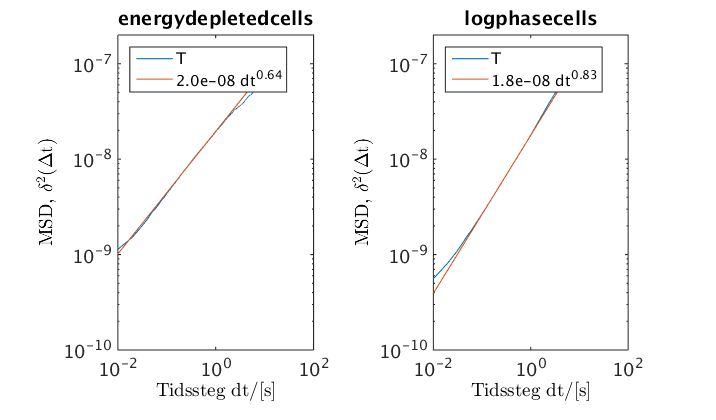
\includegraphics[width=.8\textwidth]{MSD_lilla_delta_alla.png}
    \caption{MSD beräknad under antagande att processen är stationär enligt \eqref{eq:lilla_delta} för energydepleted- och logphaseceller. Ett potenssamband har anpassats för att kunna göra jämförelser med teorin i tidigare avsnitt.}
    \label{fig:MSD_ld}
\end{figure}
\todo{Strecka anpassning för att tydligare se data}
\begin{figure}
    \centering
    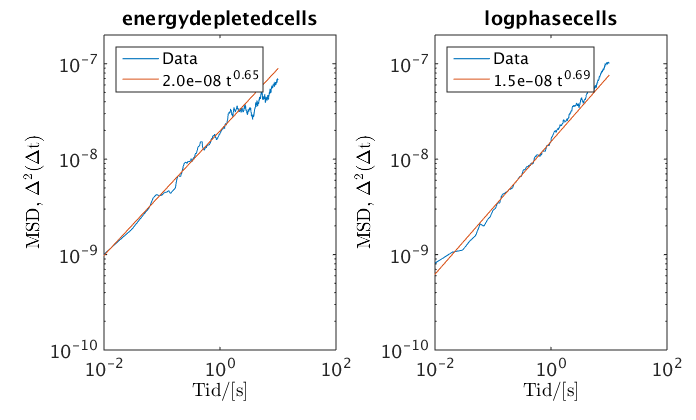
\includegraphics[width=.8\textwidth]{MSD_stora_delta_alla.png}
    \caption{MSD beräknat genom positionsförändring jämfört med startögonblicket efter $\Delta$t sekunder, beräknat enligt \eqref{eq:stora_delta}. Från potenssambandsanpassningen ses att exponenten för logphasecellerna skiljer sig väsentligt åt mellan $\Delta^2$ och $\delta^2$, se figur \ref{fig:MSD_ld} medan exponenterna för energydepleted-cellerna sammanfaller nästan exakt. Detta tyder på att de sistnämnda cellerna undergår en mer stationär process.}
    \label{fig:MSD_sd}
\end{figure}

\begin{figure}\centerline{
\subfigure[][]{
\resizebox{0.5\textwidth}{!}{% GNUPLOT: LaTeX picture with Postscript
\begingroup
  \makeatletter
  \providecommand\color[2][]{%
    \GenericError{(gnuplot) \space\space\space\@spaces}{%
      Package color not loaded in conjunction with
      terminal option `colourtext'%
    }{See the gnuplot documentation for explanation.%
    }{Either use 'blacktext' in gnuplot or load the package
      color.sty in LaTeX.}%
    \renewcommand\color[2][]{}%
  }%
  \providecommand\includegraphics[2][]{%
    \GenericError{(gnuplot) \space\space\space\@spaces}{%
      Package graphicx or graphics not loaded%
    }{See the gnuplot documentation for explanation.%
    }{The gnuplot epslatex terminal needs graphicx.sty or graphics.sty.}%
    \renewcommand\includegraphics[2][]{}%
  }%
  \providecommand\rotatebox[2]{#2}%
  \@ifundefined{ifGPcolor}{%
    \newif\ifGPcolor
    \GPcolorfalse
  }{}%
  \@ifundefined{ifGPblacktext}{%
    \newif\ifGPblacktext
    \GPblacktexttrue
  }{}%
  % define a \g@addto@macro without @ in the name:
  \let\gplgaddtomacro\g@addto@macro
  % define empty templates for all commands taking text:
  \gdef\gplbacktext{}%
  \gdef\gplfronttext{}%
  \makeatother
  \ifGPblacktext
    % no textcolor at all
    \def\colorrgb#1{}%
    \def\colorgray#1{}%
  \else
    % gray or color?
    \ifGPcolor
      \def\colorrgb#1{\color[rgb]{#1}}%
      \def\colorgray#1{\color[gray]{#1}}%
      \expandafter\def\csname LTw\endcsname{\color{white}}%
      \expandafter\def\csname LTb\endcsname{\color{black}}%
      \expandafter\def\csname LTa\endcsname{\color{black}}%
      \expandafter\def\csname LT0\endcsname{\color[rgb]{1,0,0}}%
      \expandafter\def\csname LT1\endcsname{\color[rgb]{0,1,0}}%
      \expandafter\def\csname LT2\endcsname{\color[rgb]{0,0,1}}%
      \expandafter\def\csname LT3\endcsname{\color[rgb]{1,0,1}}%
      \expandafter\def\csname LT4\endcsname{\color[rgb]{0,1,1}}%
      \expandafter\def\csname LT5\endcsname{\color[rgb]{1,1,0}}%
      \expandafter\def\csname LT6\endcsname{\color[rgb]{0,0,0}}%
      \expandafter\def\csname LT7\endcsname{\color[rgb]{1,0.3,0}}%
      \expandafter\def\csname LT8\endcsname{\color[rgb]{0.5,0.5,0.5}}%
    \else
      % gray
      \def\colorrgb#1{\color{black}}%
      \def\colorgray#1{\color[gray]{#1}}%
      \expandafter\def\csname LTw\endcsname{\color{white}}%
      \expandafter\def\csname LTb\endcsname{\color{black}}%
      \expandafter\def\csname LTa\endcsname{\color{black}}%
      \expandafter\def\csname LT0\endcsname{\color{black}}%
      \expandafter\def\csname LT1\endcsname{\color{black}}%
      \expandafter\def\csname LT2\endcsname{\color{black}}%
      \expandafter\def\csname LT3\endcsname{\color{black}}%
      \expandafter\def\csname LT4\endcsname{\color{black}}%
      \expandafter\def\csname LT5\endcsname{\color{black}}%
      \expandafter\def\csname LT6\endcsname{\color{black}}%
      \expandafter\def\csname LT7\endcsname{\color{black}}%
      \expandafter\def\csname LT8\endcsname{\color{black}}%
    \fi
  \fi
  \setlength{\unitlength}{0.0500bp}%
  \begin{picture}(4250.00,4534.00)%
    \gplgaddtomacro\gplbacktext{%
      \csname LTb\endcsname%
      \put(860,640){\makebox(0,0)[r]{\strut{}$10^{-9}$}}%
      \csname LTb\endcsname%
      \put(860,2228){\makebox(0,0)[r]{\strut{}$10^{-8}$}}%
      \csname LTb\endcsname%
      \put(860,3815){\makebox(0,0)[r]{\strut{}$10^{-7}$}}%
      \csname LTb\endcsname%
      \put(980,440){\makebox(0,0){\strut{} 0,01}}%
      \csname LTb\endcsname%
      \put(1950,440){\makebox(0,0){\strut{} 0,1}}%
      \csname LTb\endcsname%
      \put(2919,440){\makebox(0,0){\strut{} 1}}%
      \csname LTb\endcsname%
      \put(3889,440){\makebox(0,0){\strut{} 10}}%
      \put(160,2466){\rotatebox{-270}{\makebox(0,0){\strut{}$1-\text{CDF}$}}}%
      \put(2434,140){\makebox(0,0){\strut{}$\Delta{t}$ /[s]}}%
    }%
    \gplgaddtomacro\gplfronttext{%
      \csname LTb\endcsname%
      \put(3020,4080){\makebox(0,0)[r]{\strut{}\footnotesize $S(\Delta{t})$ energydepleted}}%
      \csname LTb\endcsname%
      \put(3020,3880){\makebox(0,0)[r]{\strut{}\footnotesize $s(\Delta{t})$ energydepleted}}%
      \csname LTb\endcsname%
      \put(3020,3680){\makebox(0,0)[r]{\strut{}\footnotesize Anpassning $\propto(\Delta{t})^{0,65}$}}%
    }%
    \gplbacktext
    \put(0,0){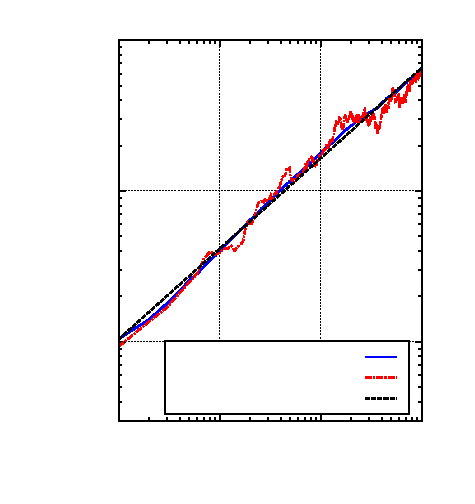
\includegraphics{MSD_ed}}%
    \gplfronttext
  \end{picture}%
\endgroup
}
}
\subfigure[][]{
\resizebox{0.5\textwidth}{!}{% GNUPLOT: LaTeX picture with Postscript
\begingroup
  \makeatletter
  \providecommand\color[2][]{%
    \GenericError{(gnuplot) \space\space\space\@spaces}{%
      Package color not loaded in conjunction with
      terminal option `colourtext'%
    }{See the gnuplot documentation for explanation.%
    }{Either use 'blacktext' in gnuplot or load the package
      color.sty in LaTeX.}%
    \renewcommand\color[2][]{}%
  }%
  \providecommand\includegraphics[2][]{%
    \GenericError{(gnuplot) \space\space\space\@spaces}{%
      Package graphicx or graphics not loaded%
    }{See the gnuplot documentation for explanation.%
    }{The gnuplot epslatex terminal needs graphicx.sty or graphics.sty.}%
    \renewcommand\includegraphics[2][]{}%
  }%
  \providecommand\rotatebox[2]{#2}%
  \@ifundefined{ifGPcolor}{%
    \newif\ifGPcolor
    \GPcolortrue
  }{}%
  \@ifundefined{ifGPblacktext}{%
    \newif\ifGPblacktext
    \GPblacktexttrue
  }{}%
  % define a \g@addto@macro without @ in the name:
  \let\gplgaddtomacro\g@addto@macro
  % define empty templates for all commands taking text:
  \gdef\gplbacktext{}%
  \gdef\gplfronttext{}%
  \makeatother
  \ifGPblacktext
    % no textcolor at all
    \def\colorrgb#1{}%
    \def\colorgray#1{}%
  \else
    % gray or color?
    \ifGPcolor
      \def\colorrgb#1{\color[rgb]{#1}}%
      \def\colorgray#1{\color[gray]{#1}}%
      \expandafter\def\csname LTw\endcsname{\color{white}}%
      \expandafter\def\csname LTb\endcsname{\color{black}}%
      \expandafter\def\csname LTa\endcsname{\color{black}}%
      \expandafter\def\csname LT0\endcsname{\color[rgb]{1,0,0}}%
      \expandafter\def\csname LT1\endcsname{\color[rgb]{0,1,0}}%
      \expandafter\def\csname LT2\endcsname{\color[rgb]{0,0,1}}%
      \expandafter\def\csname LT3\endcsname{\color[rgb]{1,0,1}}%
      \expandafter\def\csname LT4\endcsname{\color[rgb]{0,1,1}}%
      \expandafter\def\csname LT5\endcsname{\color[rgb]{1,1,0}}%
      \expandafter\def\csname LT6\endcsname{\color[rgb]{0,0,0}}%
      \expandafter\def\csname LT7\endcsname{\color[rgb]{1,0.3,0}}%
      \expandafter\def\csname LT8\endcsname{\color[rgb]{0.5,0.5,0.5}}%
    \else
      % gray
      \def\colorrgb#1{\color{black}}%
      \def\colorgray#1{\color[gray]{#1}}%
      \expandafter\def\csname LTw\endcsname{\color{white}}%
      \expandafter\def\csname LTb\endcsname{\color{black}}%
      \expandafter\def\csname LTa\endcsname{\color{black}}%
      \expandafter\def\csname LT0\endcsname{\color{black}}%
      \expandafter\def\csname LT1\endcsname{\color{black}}%
      \expandafter\def\csname LT2\endcsname{\color{black}}%
      \expandafter\def\csname LT3\endcsname{\color{black}}%
      \expandafter\def\csname LT4\endcsname{\color{black}}%
      \expandafter\def\csname LT5\endcsname{\color{black}}%
      \expandafter\def\csname LT6\endcsname{\color{black}}%
      \expandafter\def\csname LT7\endcsname{\color{black}}%
      \expandafter\def\csname LT8\endcsname{\color{black}}%
    \fi
  \fi
  \setlength{\unitlength}{0.0500bp}%
  \begin{picture}(4250.00,4534.00)%
    \gplgaddtomacro\gplbacktext{%
      \csname LTb\endcsname%
      \put(860,1397){\makebox(0,0)[r]{\strut{}$10^{-1}$}}%
      \csname LTb\endcsname%
      \put(860,2845){\makebox(0,0)[r]{\strut{}$10^{0}$}}%
      \csname LTb\endcsname%
      \put(860,4293){\makebox(0,0)[r]{\strut{}$10^{1}$}}%
      \csname LTb\endcsname%
      \put(980,440){\makebox(0,0){\strut{} 0,01}}%
      \csname LTb\endcsname%
      \put(1950,440){\makebox(0,0){\strut{} 0,1}}%
      \csname LTb\endcsname%
      \put(2919,440){\makebox(0,0){\strut{} 1}}%
      \csname LTb\endcsname%
      \put(3889,440){\makebox(0,0){\strut{} 10}}%
      \put(160,2466){\rotatebox{-270}{\makebox(0,0){\strut{}MSD $/\left[\text{godt. längdenhet}^2\right]$}}}%
      \put(2434,140){\makebox(0,0){\strut{}$\Delta{t}$ /[s]}}%
    }%
    \gplgaddtomacro\gplfronttext{%
      \csname LTb\endcsname%
      \put(3226,1253){\makebox(0,0)[r]{\strut{}\footnotesize $S(\Delta{t})$, log-fas}}%
      \csname LTb\endcsname%
      \put(3226,1053){\makebox(0,0)[r]{\strut{}\footnotesize $s(\Delta{t})$, log-fas}}%
      \csname LTb\endcsname%
      \put(3226,853){\makebox(0,0)[r]{\strut{}\footnotesize Anpassning $\propto(\Delta{t})^{0,8}$}}%
    }%
    \gplbacktext
    \put(0,0){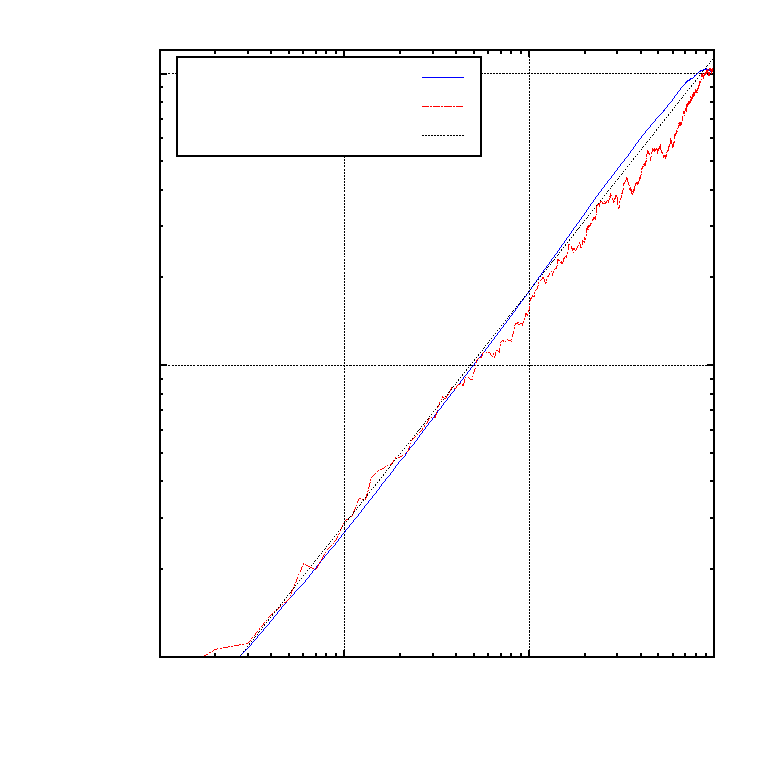
\includegraphics{MSD_lp}}%
    \gplfronttext
  \end{picture}%
\endgroup
}
}}
\caption{}
\label{fig:MSD}
\end{figure}


Båda dessa beräkningar har utförts för given data och exponentens värde i sambandet mellan MSD och tid skiljer sig olika mycket åt för energydepleted (dvala) och logphase (aktiva) cellerna, se figur \ref{fig:MSD_ld} och \ref{fig:MSD_sd}. Mest relevant är kanske att jämföra exponenterna i det anpassade potenssambandet som för energydepleted cellerna blev 0,64 för $S$ och 0,65 för $s$. Med denna lilla skillnad ter sig partikelrörelsen för celler i dvala vara en ganska stationär process, något som inte lika säkert kan uttalas för resultatet från de aktiva logphase cellerna. Där blev exponenten 0,83 för $S$ och 0,69 för $s$. En väsentlig skillnad, men hurvida resultatet säger något om att processen är stationär eller ej kan ej uttalas utan att hänsyn tagits till relevanta felgränser.

Från dessa beräknade MSD-plottar kan man även avläsa att logphase-cellerna har högre exponent  för både $S$ och $s$ vilket tyder på att partiklarna sprids ut snabbare i dessa cellers cytoplasma jämfört med energydepleted-cellerna. Ökad aktivitet i cellen tycks därmed ge ökad diffusion.



\begin{comment} %För att dölja för fackspråk
\section{Spektraltäthet och brushantering}
Ett annat verktyg för att undersöka partilarnas rörelser är att titta på vad för spektraläthet partiklarnas position har. Spektraltätheten erhålls genom att ta Fouriertransformen av partikelns position som funktion av tid. På så sätt erhålls ett mått på hur mycket av varje frekvens som finns. Detta kan vara användbart på flera olika sätt; bland annat ger det ett annat sätt att \todo{Jag vet fortfarande inte hur man gör här}ta fram hur MSD:n beter sig, men spektraltätheten kan också användas för att 

Om man 
\begin{equation}
\hat{x} = x + \sigma\eta
\end{equation}


\todo[inline]{Mer kommer sen.}

Ett annat sätt att upptäcka bruset i en mätning är att titta på 


\subsection{Resultat}


\end{comment}


\section{Anisotropi}
Om man misstänker att cellens inre struktur påverkar partikelrörelserna skulle eventuell anisotropi kunna ge ett bidrag till dessa. Alltså ifall det finns föredragna riktningar för partikeln att röra sig i. Ett sätt att undersöka detta är genom att betrakta koordinaternas \todo{Anpassa till kap. 2!}kovarianstensor som är en tensor med de olika koordinaternas statistiska andramoment:
\begin{equation}
C_{ij} = \frac{1}{N} \sum_{n=1}^{N} r_i^{(n)}r_j^{(n)},
\end{equation}
där $r_i^{(n)}$ är den $i$:te koordinaten ($x$ eller $y$) i den $n$:te datapunkten. Man kan också skriva $C$ på matrisform enligt
\begin{equation}
C=
\begin{bmatrix} \label{eq:C_matrix}
\ev{x^2} & \ev{xy}\\
\ev{yx} & \ev{y^2}
\end{bmatrix}.
\end{equation}

Notera hur snarlik $C$ är med tröghetstensorn för en kropps olika tröghetsmoment som uppkommer i mekaniken. Och precis som i mekaniken kan man hitta två principalaxlar genom att ta fram dess egenvektorer och diagonalisera tensorn. I mekaniken svarar principalaxlarna mot de riktningar av rörelsemängdsmoment som är oberoende av rotation längs andra axlar. I de här statistiska sammanhangen finns det en liknande tolkning nämligen att principalaxlarna svarar mot de riktningar i cellen där rörelserna är oberoende av varandra. Egenvärdena i dessa två riktningarna svarar mot variansen i den oberoende koordinaten längs med den riktningen.

\todo[inline]{Byta till assymetrimåttet: $A=\dfrac{\ev{(\lambda_1 - \lambda_2)^2}}{\ev{(\lambda_1 + \lambda_2)^2}}$. }

För att ur kovarianstensorn få ut ett mått på hur isotrop partikelns position är kan man undersöka kvoten
\begin{equation}
\varLambda = \frac{\lambda_2}{\lambda_1} >1
\end{equation} \todo{Kallas "shape parameter"?}
mellan det större, $\lambda_2$, och det mindre, $\lambda_1$,  egenvärdet till $C$. Egenvärdena själva svarar som sagt mot variansen i de olika riktningarna, vilket motsvarar hur mycket partikeln har rört sig i respektive rikting. Hade positionerna varit helt isotropt fördelade så hade alltså $\varLambda=1$. 

Något som också kan ge en vink om hur asymmetrisk partikelns rörelse är, är följande asymmetrimått \cite{Hong_asymmetri1998}
\begin{equation}
A=\dfrac{\ev{(\lambda_1 - \lambda_2)^2}}{\ev{(\lambda_1 + \lambda_2)^2}},
\end{equation}
kallat \todo{Översätta till svenska?} \emph{asphericity} \cite{Rudnick_Asphericity1986}. A=0 svarar här mot att rörelsen i snitt sker helt cirkulärt symmetriskt medan A=1 ger att rörelsen endast sker i en riktning, längs en linje. Man kan enkelt visa att egenvärdena till \todo{Eller gyration tensorn?}kovarianstensorn i ekvation \todo{Dra bort medelvärde?} \eqref{eq:C_matrix} uppfyller
\begin{align}
    \lambda_1+\lambda_2 &= \ev{x^2}+\ev{y^2} \\
    \abs{\lambda_1-\lambda_2} &= \sqrt{(\ev{x^2}-\ev{y^2})^2 + 4\ev{xy}^2}.
\end{align} %&= för att den ska linjera efter "="
För en given fördelningsfunktion med ändliga moment blir det därmed nu möjligt att beräkna denna kvot teoretiskt.

För en obegränsad slumpvandring i $d$ dimensioner fås 
\begin{equation} \label{eq:Asphericity_Brownian}
    A_d=\frac{2(d+2)}{5d+4}.
\end{equation}
och för två dimensioner $d=2$ fås därmed $A=\nicefrac{4}{7}$. Detta innebär att även långvariga slumpvandringar i snitt kommer att uppvisa viss asymmetri mellan de två riktningarna. \todo{Kan kanske formuleras bättre?}

För fBm fås en approximativ formel i två dimensioner i gränsen där antalet mätpunkter blir mycket stort ~\cite{Hong_asymmetri1998}
\begin{equation} \label{eq:A_fBm}
A=2-\frac{\frac{1}{2(H+1)^2}}{\frac{1}{2(H+1)^2}+\frac{2H+1}{4(4H+1)}-\frac{1}{4H+3}-\frac{\Gamma^2(2H+2)}{\Gamma(4H+4)}},
\end{equation}
där $H$ är Hurst parametern som karakteriserar rörelsen och $\Gamma$ gamma-funktionen. För $H=\nicefrac{1}{2}$ fås en vanlig brownsk rörelse med motsvarande  asymmetrimått $A=\nicefrac{4}{7}$ vilket stämmer överens med ekvation \eqref{eq:Asphericity_Brownian}. Samma värde fås även approximativt för CTRW-modellen \cite{Ernst_ACTRW2012} då denna rörelse vid varje tidsögonblick ser ut som brownsk rörelse. \todo{Kolla upp}.

%Även http://iopscience.iop.org/article/10.1088/0305-4470/19/4/004/pdf

\subsection{Simulering} %Något om egenvärdes kvoter i titel
Eftersom en mätning bara kan bestå av ett ändligt antal datapunkter kan även en äkta, isotrop Brownsk rörelse ge upphov till $\varLambda>1$. Vidare är \emph{kvoten} mellan egenvärden inte linjär, vilket gör en teoretisk analys av fördelningarna mycket svår. För att ändå kunna säga något om den riktiga datan kan man ganska enkelt ta fram en fördelning för $\varLambda$ för några olika modeller genom simulering. 

De modeller som testats är en vanlig Wienerprocess, en Wienerprocess med ett ''mätbrus'' pålagt och en Ornstein–Uhlenbeck-process. Från dessa processer samt från datan över partikelrörelsen erhölls olika fördelningar av egenvärdeskvoter. 
%För att vara konsekvent vid beräkningen av fördelningarna användes alltid kvoten av det större egenvärdet delat med det mindre. Detta ger att $\varLambda$ kan anta värden från $1$ och uppåt. 

Wienerprocessen simulerade fram partikelns position i varje ny tidpunkt genom att gå ett normalfördelat steg från positionen i den förra tidpunkten. Detta kan skrivas som
\begin{equation}\label{eq:sim_wiener}
x_{i+1} = x_i + \delta 
\qcomma  \delta \sim N(0, \sigma)
\end{equation}
och där $x_1=0$. Sedan gör man samma sak för $y$. Eftersom $\varLambda$ ger ett mått på hur mycket partikeln \emph{föredrar en viss riktning}, finner man att värdet på $\sigma$ inte påverkar fördelningen -- så länge $\sigma$ är samma för både $x$ och $y$. Detta blir uppenbart när man tänker på att \eqref{eq:sim_wiener} kan skrivas som 
\begin{equation}
x_{i+1} =\sigma\,\hat{x}_{i+i} = \sigma\,\left( \hat{x}_i + \hat{\delta} \right) 
\qcomma  \hat{\delta} \sim N(0, 1).
\end{equation}
Alltså att $\sigma$ bara är en multiplikativ konstant framför positionen.

För att istället simulera en Wienerprocess med mätbrus användes \eqref{eq:sim_wiener} för att först simulera själva Wienerprocessen för att sedan \emph{efteråt} addera en slumpad brusterm $\eta \sim N(0, \sigma')$ till varje $x_i$. Den väsentliga skillnaden mot en ren Wienerprocess är att mätbruset $\eta$ inte påverkar nästkommande position. Till skillnad från den rena Wienerprocessen så kommer värdena på $\sigma$ och $\sigma'$ att påverka $\varLambda$, men enligt samma argument som ovan kommer bara kvoten $\nicefrac{\sigma'}{\sigma}$ vara det som påverkar. Detta gör att simuleringarna med mätbrus går att genomföra med olika värden på parametern $\nicefrac{\sigma'}{\sigma}$ för att få olika fördelningar av $\varLambda$. 

Ornstein-Uhlenbeck-processen i \eqref{eq:SDE_o-u} simulerades genom att använda derivatan för tidsutveckling och genom att sätta $\bar{x}=0$. Man får då
\begin{equation}
x_{i+1} = x_i + \Delta{t}\,\pd_{t}x  = (1-k) x_i +  \delta 
\qcomma  \delta \sim N(0, \sigma),
\end{equation}
där $x_1=0$. Notera här att den styrande parametern i simuleringarna är $k=\gamma\Delta{t}$, samt att $\sigma$ på samma sätt som för den rena Wienerprocessen kan väljas godtyckligt utan att påverka $\varLambda$. 

Eftersom resultatet för Asymmetrimåttet i ekvation \eqref{eq:A_fBm} gäller för riktigt långa mätningar medan den data som analyseras i detta arbete är ganska begränsad kan man försöka simulera fram sannolikheter istället. Genom att simulera många mätserier för samma antal steg och antal partiklar som i datan kan man bedöma sannolikheten att det framräknade asymmetrimåttet till exempel skulle ha kommit från en ren klassisk brownsk rörelse. 

\subsection{Resultat -- partiklarna är mer isotropa än Wienerprocessen}
En anledning till att kolla om en tydlig asymmetri kan uttydas ur datan över partiklarnas rörelse är att bedöma hurvida man istället för de givna x- och y-koordinaterna bör gå över till tangential- och normalkoordinater. Eftersom ingen sådan uttalad assymetri verkar finnas borde koordinatsystemet lämnas som det är.

Genom att spela upp datan över partikelpositionerna som en film blir det tydligt att vissa partiklar stöter på större strukturer i cytoplasman som de inte kan rubba ur vägen utan måste ta sig runt. För dessa partiklar ter sig cytoplasman alltså inte helt isotrop. \todo{Vad kan man säga mer här?}


%Mer isotropt än vid brownsk rörelse. Påverkas kanske av cellens inre utformning och hålls på plats


\begin{comment}%För att gömma för fackspråk
\section{Storleksberoende}

%Om värdena skiljer sig åt väsentligt för små och stora partiklar -> CTRW mer trolig. 

\subsection{Resultat}
\end{comment}


\section{Diskussion}
\todo[inline]{Inga tomma rubriker!}

\subsection{Ornstein-Uhlenbeck-modellen}
\todo[inline]{Varsågod att ändra så mycket ni vill.}


%Om sambandet mellan intensitet och partikelstorleken påverkar resultatet

%Byter man till normal- och tangential-koordinater bygger man in ett bias som påverkar resultaten till att det verkar finnas egenskaper som egentligen inte finns. 
%Av slumpskäl kommer vissa vägar att vara mer raka än andra medan andra får mer symmetriska banor.


%Bara en liten kodsnutt som behövs när man kompilerar lokalt
%%% Local Variables: 
%%% mode: latex
%%% TeX-master: "00main.tex"
%%% End: 


\chapter{Strängars rörelse i vätskor}

%\subsubsection{Strängrörelser inom cellen}
Aktinfilament är polymerer vilka utgör en viktig byggsten för cellens cytoskelett och transportväg för motorprotein vilka formar och bidrar till cellens utseende, dynamik och stadga. För att kunna ge en mer detaljerad beskrivning av dessa egenskaper är studien av enstaka aktinfilaments dynamik av stort intresse. I detta arbete har olika dynamiska egenskaper för aktinfilament studerats, både för filament som fluktuerar fritt i en vätska och filament instängda i en rektangulär kvasi-2D mikrokanal. Mikrokanalen är till för att simulera beteendet hos aktinfilament i cytoskelettet där det omges av andra filament och därmed har en begränsad möjlighet till rörelse.

%\section{}


\section{Modeller för strängrörelser}
Aktinfilamenten precis som tidigare studerade partiklar påverkas av diffusionsprocessen inuti celler och således krävs stokastiska modeller för att beskriva rörelsen. En vanligt använd modell inom polymerfysiken är Worm Like Chain-model som beskrivs nedan. Vidare studeras en modell i form av en langevinekvation med en brusterm som innehar brownsk karaktär.

\subsection{Worm Like Chain-model}
Worm like chain modellen \cite{Milstein2013} (WLC) är en modell som ämnar beskriva fluktuationerna hos en semi-flexibel polymer. I modellen antas att polymeren är helt oelastisk, enbart påverkas av termiskt brus och styv på små längdskalor. Då polymeren fluktuerar fritt utan att vara instängd i en mikrokanal ges en minimalistisk WLC beskrivning av att filamentets fluktuationer regleras av böjningsenergin. För en polymer av $N$ segment vardera med riktning \textbf{r}$_i$ och längd $\abs{r_{i}}=l$ samt polymerens böjstyvhet $\kappa$ ges böjningsenergin av 
\begin{equation}
    H = -\kappa\sum_{i=1}^{N}\textbf{r}_{i}\cdot \textbf{r}_{i+1}.
\end{equation}
Maximalt bidrag till energin från två på varandra följande segment fås alltså om dessa har antiparallell riktning. Givet identiteten $\textbf{r}_{i}\cdot\textbf{r}_{i+1}=\frac{2l^2-(\textbf{r}_{i+1}-\textbf{r}_{i})^2}{2}$ kan summan skrivas om som en integral i gränsen då $N \rightarrow \infty$, $\kappa\to\infty$, $l \rightarrow 0$ samt produkten \todo{Någon annan variabelnamn än $\xi$?}$\kappa l=\xi$ finit 
\begin{equation}
    H=\frac{\xi}{2}\int_{0}^{L}ds(\partial_{s}\textbf{t}(s))^2
\end{equation}
där $\textbf{t}(s)$ är enhetstangentvektorn längs polymeren parametriserad med båglängden. Detta är den kontinuerliga WLC modellen \cite{Fixman_WLC1973} vilket ger en bra approximation av en polymer där längden hos enstaka molekyler kan försummas. \todo{Den diskreta modellen heter väl FJC=freely jointed chain? Inte diskret WLC?} Korrelationen mellan två tangentvektorer medelvärdsbildat över tid ges av \cite{Landau1958}:
\begin{equation}
\ev{\textbf{t}(s)\textbf{t}(s+\Delta s)}=e^{-\frac{\abs{\Delta s}}{2L_{p}}}
\end{equation}
Där $L_{p}=\frac{\xi}{k_{B}T}$ är kvoten mellan styvheten hos polymeren och termiska energin hos fluiden. Denna kallas \emph{persistent length} och ger ett mått på hur snabbt tangentkorrelationen avtar längs polymeren. I fallet då $\nicefrac{L_{p}}{L}>1$ sägs polymeren vara styv. Ytterligare kan ett rumsligt medelvärde av dessa tangentkorrelationer beräknas. Beteckna denna rumsliga medelvärdesbildning med ett heldraget streck. Tangentkorrelationen kommer då enbart bero på avståndet mellan tangentvektorerna, $\Delta s$, och kan definieras som
\begin{equation}
\label{tangkorr}
    \ev{cos\theta(\Delta s)}\equiv\overline{\ev{\mathbf{t}(s)\mathbf{t}(s+\Delta s)}}.
\end{equation}
Denna minimalistiska WLC modell är intressant då den utgår från att strängen kan fluktuera fritt. Givet ett dataset av fria strängar samt strängar placerade i mikrokanaler kan påverkan av denna studeras. En sträng i en mikrokanal antas uppleva en återställande kraft riktad mot centrum av kanalen. Det resulterar i att tangentkorrelationen är mer ihärdig.

\subsection{WLC-modell för sträng i mikrokanal}

En mer sofistikerad modell kan konstrueras med avseende till mikrokanalens egenskaper och dess dynamik. Då interaktionen mellan strängen och kanalens väggar beskrivs som rent sterisk \cite{Koster_etal2007} kan denna approximeras med en parabolisk potential. Därmed införs en återställande kraft $F \propto z(s)^2$ där $z(s)$ svarar mot avståndet vinkelrätt mot centrum av kanalen. \emph{Persistent length} definerades tidigare som den karakterisktiska längdskalan på vilket termiska fluktuationerna kan ge upphov till signifikant böjning av strängen. Eftersom potentialen fixerar strängen längs kanalens centrum fås \emph{persistent length} mycket stor $\nicefrac{L_{p}}{L}\gg 1$. Det resulterar i att krökninsenergin enligt den tidigare härledda WLC-modellen blir försummbar \cite{PhysRevE.60.4671} $\ev{(\partial_{s}\mathbf{t})^2}\ll 1$ och \todo{kanske ge bättre förklaring} krökningsenergin defineras istället med avseende på strängens avvikelse relativt kanalens centrum. Hamiltonianen fås som
\begin{equation}
\label{Hkanal}
    H=\int_{0}^{L}ds[\kappa(\partial_{s}^2\mathbf{t}(s))^2+ \gamma z(s)^2],
\end{equation}
där $\gamma$ är en positiv konstant vilket representerar styrkan hos potentialen.\\
Tangentkorrelationen för en sträng i en mikrokanal kan nu beräknas genom att betrakta \eqref{Hkanal}. Hamiltonianen representerar energin hos strängen, då denna antas utvecklas i tiden fås följande langevin ekvation
\todo{jobba på övergången}
%Betrakta en semi-flexibel polymer utsatt för ett stokastiskt termiskt brus. Polymerens jämviktstillstånd sätts till att vara fixerad längs $z$-axeln med fluktuationer i $x$/$y$ - planet. Då fluktuationerna är små relativt polymeren kan de approximeras som oberoende i $x$/$y$ -planet, låt $A(t,z)$ beteckna fluktuationerna i x-riktningen. Då polymerens jämviktstillstånd tillstånd minimerar dess potentiella energi införs en parabolisk potential för att återställa avvikelser från detta läge. Likt WLC modellen lagras även potentiell energi i formen av krökning av polymeren. Tidsutvecklingen av $A(t,z)$ ges då av
\begin{equation}
\label{mans}
    \partial_{t}z(t,z)=-\gamma z(t,z)+\kappa \partial_{x}^{2}z(t,z)+\sigma \partial_{t}W(t,z)
\end{equation}
Där $W(t,z)$ är en stokastisk brusterm och $\sigma$ ett posistivt reellt tal proportionellt mot dess intensitet.\\
Definera fouriertransformation som \todo{Låta $s\to k$, ev förvirrning med båglängdsparametern?}
\begin{equation}
    \hat{A}(t,s)=\int_{-\infty}^{\infty}\dd{z} A(t,z)\ee^{-\ii sz}
\end{equation}
Genom fouriertransformation av \eqref{mans} fås en ordinär stokastisk differentialekvation
\begin{equation}
        \partial_{t}\hat{A}(t,s)=-\left(\gamma+\alpha s^2\right)\hat{A}(t,z)+\sigma \partial_{t}\hat{W}(t,z)
\end{equation}
vars lösning enkelt kan visas vara
\begin{equation}
        \hat{A}(t,s)=\ee^{-(\gamma+\alpha s^2)t}\left(\hat{A}(0,s)+\sigma\int_{0}^{t}\dd\tau \ee^{(\gamma+\alpha s^2)\tau}\partial_{t}\hat{W}(\tau,z)\right)
\end{equation}
Tvåpunktskorrelationen för den fouriertransformerade stokastiska variabeln $\hat{A}(t,s)$ kan då beräknas till
\begin{equation}
\begin{aligned}
    \ev{\hat{A}(t,s)\hat{A}(t',s')} =& \ev{\hat{A}(0,s)\hat{A}(0,s')} \ee^{-(\gamma+\alpha s^2)(t+t')}\\ 
    &+ \sigma^2 \int_{0}^{t}\int_{0}^{t'}\dd\tau\dd\tau' \ee^{(\gamma+\alpha s^2)(\tau+\tau')} \ev{\partial_{t}\hat{W}(\tau,s)\partial_{t}\hat{W}(\tau',s')}
\end{aligned}
\end{equation}
Definera nu $\Delta t=t-t'$ samt $\Delta s=s-s'$ och betrakta korrelationen i gränsen då $t,t'\rightarrow\infty$ medan $\Delta t$ hålls finit. Då fås
\begin{equation}\label{jobbig}
     \ev{\hat{A}(t,s)\hat{A}(t',s')}=\sigma^2\int_{0}^{t}\int_{0}^{t'}\dd\tau\dd\tau'\ee^{(\gamma+\alpha s^2)(\tau+\tau')}\ev{\partial_{t}\hat{W}(\tau,s)\partial_{t}\hat{W}(\tau',s')}
\end{equation}
Notera att integranden i \eqref{jobbig} är korrelationen av fouriertransformerade brustermen $W(t,z)$. Då termiska bruset antas vara brownskt definieras det av följande tvåpunktskorrelation
\begin{equation}\label{brus}
    \ev{\partial_{t}W(t,z)\partial_{t}W(t',z')}=\delta(t- t')\delta(z-z')
\end{equation}
Fouriertransformation av \eqref{brus} ger \todo{ekvation 4.13+4.14 kanske kan skippas om man vill minska antal ekvationer.}
\begin{equation}
    \ev{\partial_{t}\hat{W}(t,s)\partial_{t}\hat{W}(t',s')}=\int_{-\infty}^{\infty}\int_{-\infty}^{\infty}\dd z \dd z'\ev{\partial_{t}W(t,z)\partial_{t}W(t',z')}\ee^{-izs}\ee^{-iz's'}
\end{equation}
Genom insättning av \eqref{brus} kan integralen i högerledet beräknas.
\begin{equation}\label{fourbrus}
    \ev{\partial_{t}\hat{W}(t,s)\partial_{t}\hat{W}(t',s')}=\delta(t-t')\int_{-\infty}^{\infty}\int_{-\infty}^{\infty}\dd z \dd z'\delta(z-z')\ee^{-i(sz+s'z')}=\delta(t-t')\delta(s+s')
\end{equation}
Insättning av \eqref{fourbrus} i \eqref{jobbig} reducerar ekvationen till en enkelintegral och tvåpunktskorrelationen i fourierrummet ges av
\begin{equation}
    \ev{\hat{A}(t,s)\hat{A}(t',s')}=\frac{\sigma^2}{2(\gamma+\alpha s^2)}\delta(s+s')\ee^{(\gamma+\alpha s^2)\abs{t-t'}}
\end{equation}
Genom invers fouriertransform fås tvåpunktskorrelationen för de rumsliga variblerna $z$,$z'$ som
\begin{equation}
    \ev{A(t,z)A(t',z')}=\frac{1}{(2\pi)^2}\int_{-\infty}^{\infty}\int_{-\infty}^{\infty}\dd s \dd s'\frac{\sigma^2}{2(\gamma+\alpha s^2)}\delta(s+s')\ee^{(\gamma+\alpha s^2)\abs{t-t'}}\ee^{-izs}\ee^{-iz's'}
\end{equation}
Förenkling av integralen kan göras genom insättning av variabeln $p$ definerad som $\frac{dp}{dk}=\sqrt{\frac{\alpha}{\gamma}}$. Tvåpunktskorrelationen kan slutligen beräknas och ges av 
\begin{equation}
\label{2korr}
    \ev{A(t,z)A(t',z')}=\frac{1}{(2\pi)^2\sqrt{\gamma\alpha}}\int_{-\infty}^{\infty}\dd p \frac{\ee^{-(1+p^2)\gamma \abs{t-t'}+\ii p\sqrt{\frac{\gamma}{\alpha}}(s-s')}}{1+p^2}.
\end{equation}
\
Givet data från strängar begränsade av en 2D-mikrokanal kan tvåpunktskorrelationen beräknas numeriskt. Då denna modell förutspår korrelationen för en sådan sträng kan resultatet användas för att bestämma konstanterna $\alpha,\gamma,\sigma$. 

Tvåpunktskorrelationen kan även betraktas i fallet då $\abs{t-t'}\equiv 0$, vilket svarar mot korrelation längs med strängen. \eqref{2korr} kan i detta fallet lösas analytiskt och fås som
\begin{equation}
\ev{A(z)A(z')}=exp(-\sqrt{\frac{\gamma}{\alpha}}\abs{z-z'}),
\end{equation}
Motsvarande \emph{Persistent length} defineras ur denna modell som $L_{p}=\sqrt{\frac{\alpha}{\gamma}}$. Notera dess beroende av dämpande termen $\gamma$. 




\section{Egenmoder}
Ett vanligt sätt att studera svängningar är att dela upp svängningarna i egenmoder. Genom en linjärkombination av dessa egenmoder kan en godtycklig svängning representeras. Anledningen till att det är intressant att studera egenmoder är på grund av att de är oberoende av varandra. Precis som \todo{beskriva mer tydligt hur data ser ut samt hur avst etc beräknas.} svängningen på en gitarrsträng kan man eventuellt dela in svängningen av en sträng i cellen som en linjärkombination av dess egenmoder. 

Metoden för att åstadkomma denna sönderläggning av strängens rörelse i egenmoder beskrivs i avsnitt \ref{sec:diskret_data} som en diagonalisering av kovariansmatrisen, där kovariansmatrisen $C$ i detta fallet byggs upp av avståndskomponenter till strängen. Hädanefter betecknas därför det transversella avståndet till strängen relativt sitt jämviktsläge $A_s(t)$ där $s$ är en diskret båglängdsparameter längs med strängen. Diagonalisering av denna kovariansmatris med hjälp av spektralsatsen leder effektivt till ett basbyte från en bas bestående av det transversella avståndet i varje $s$ längs strängen, till en bas bestående av egenmoderna för strängen. Egenvärdena till kovariansmatrisen ger ett mått på hur mycket av strängens rörelse som byggs upp av motsvarande egenmod. Genom att projicera strängens rörelse på ett fåtal av de egenmoder med ''störst''\todo{bättre ord} egenvärde förenklas analysen\cite{Shlens_PCA2014}; karakteristiska egenskaper för varje egenmod kan undersökas separat. 



\subsection{Resultat -- }

\begin{figure}
    \centering
    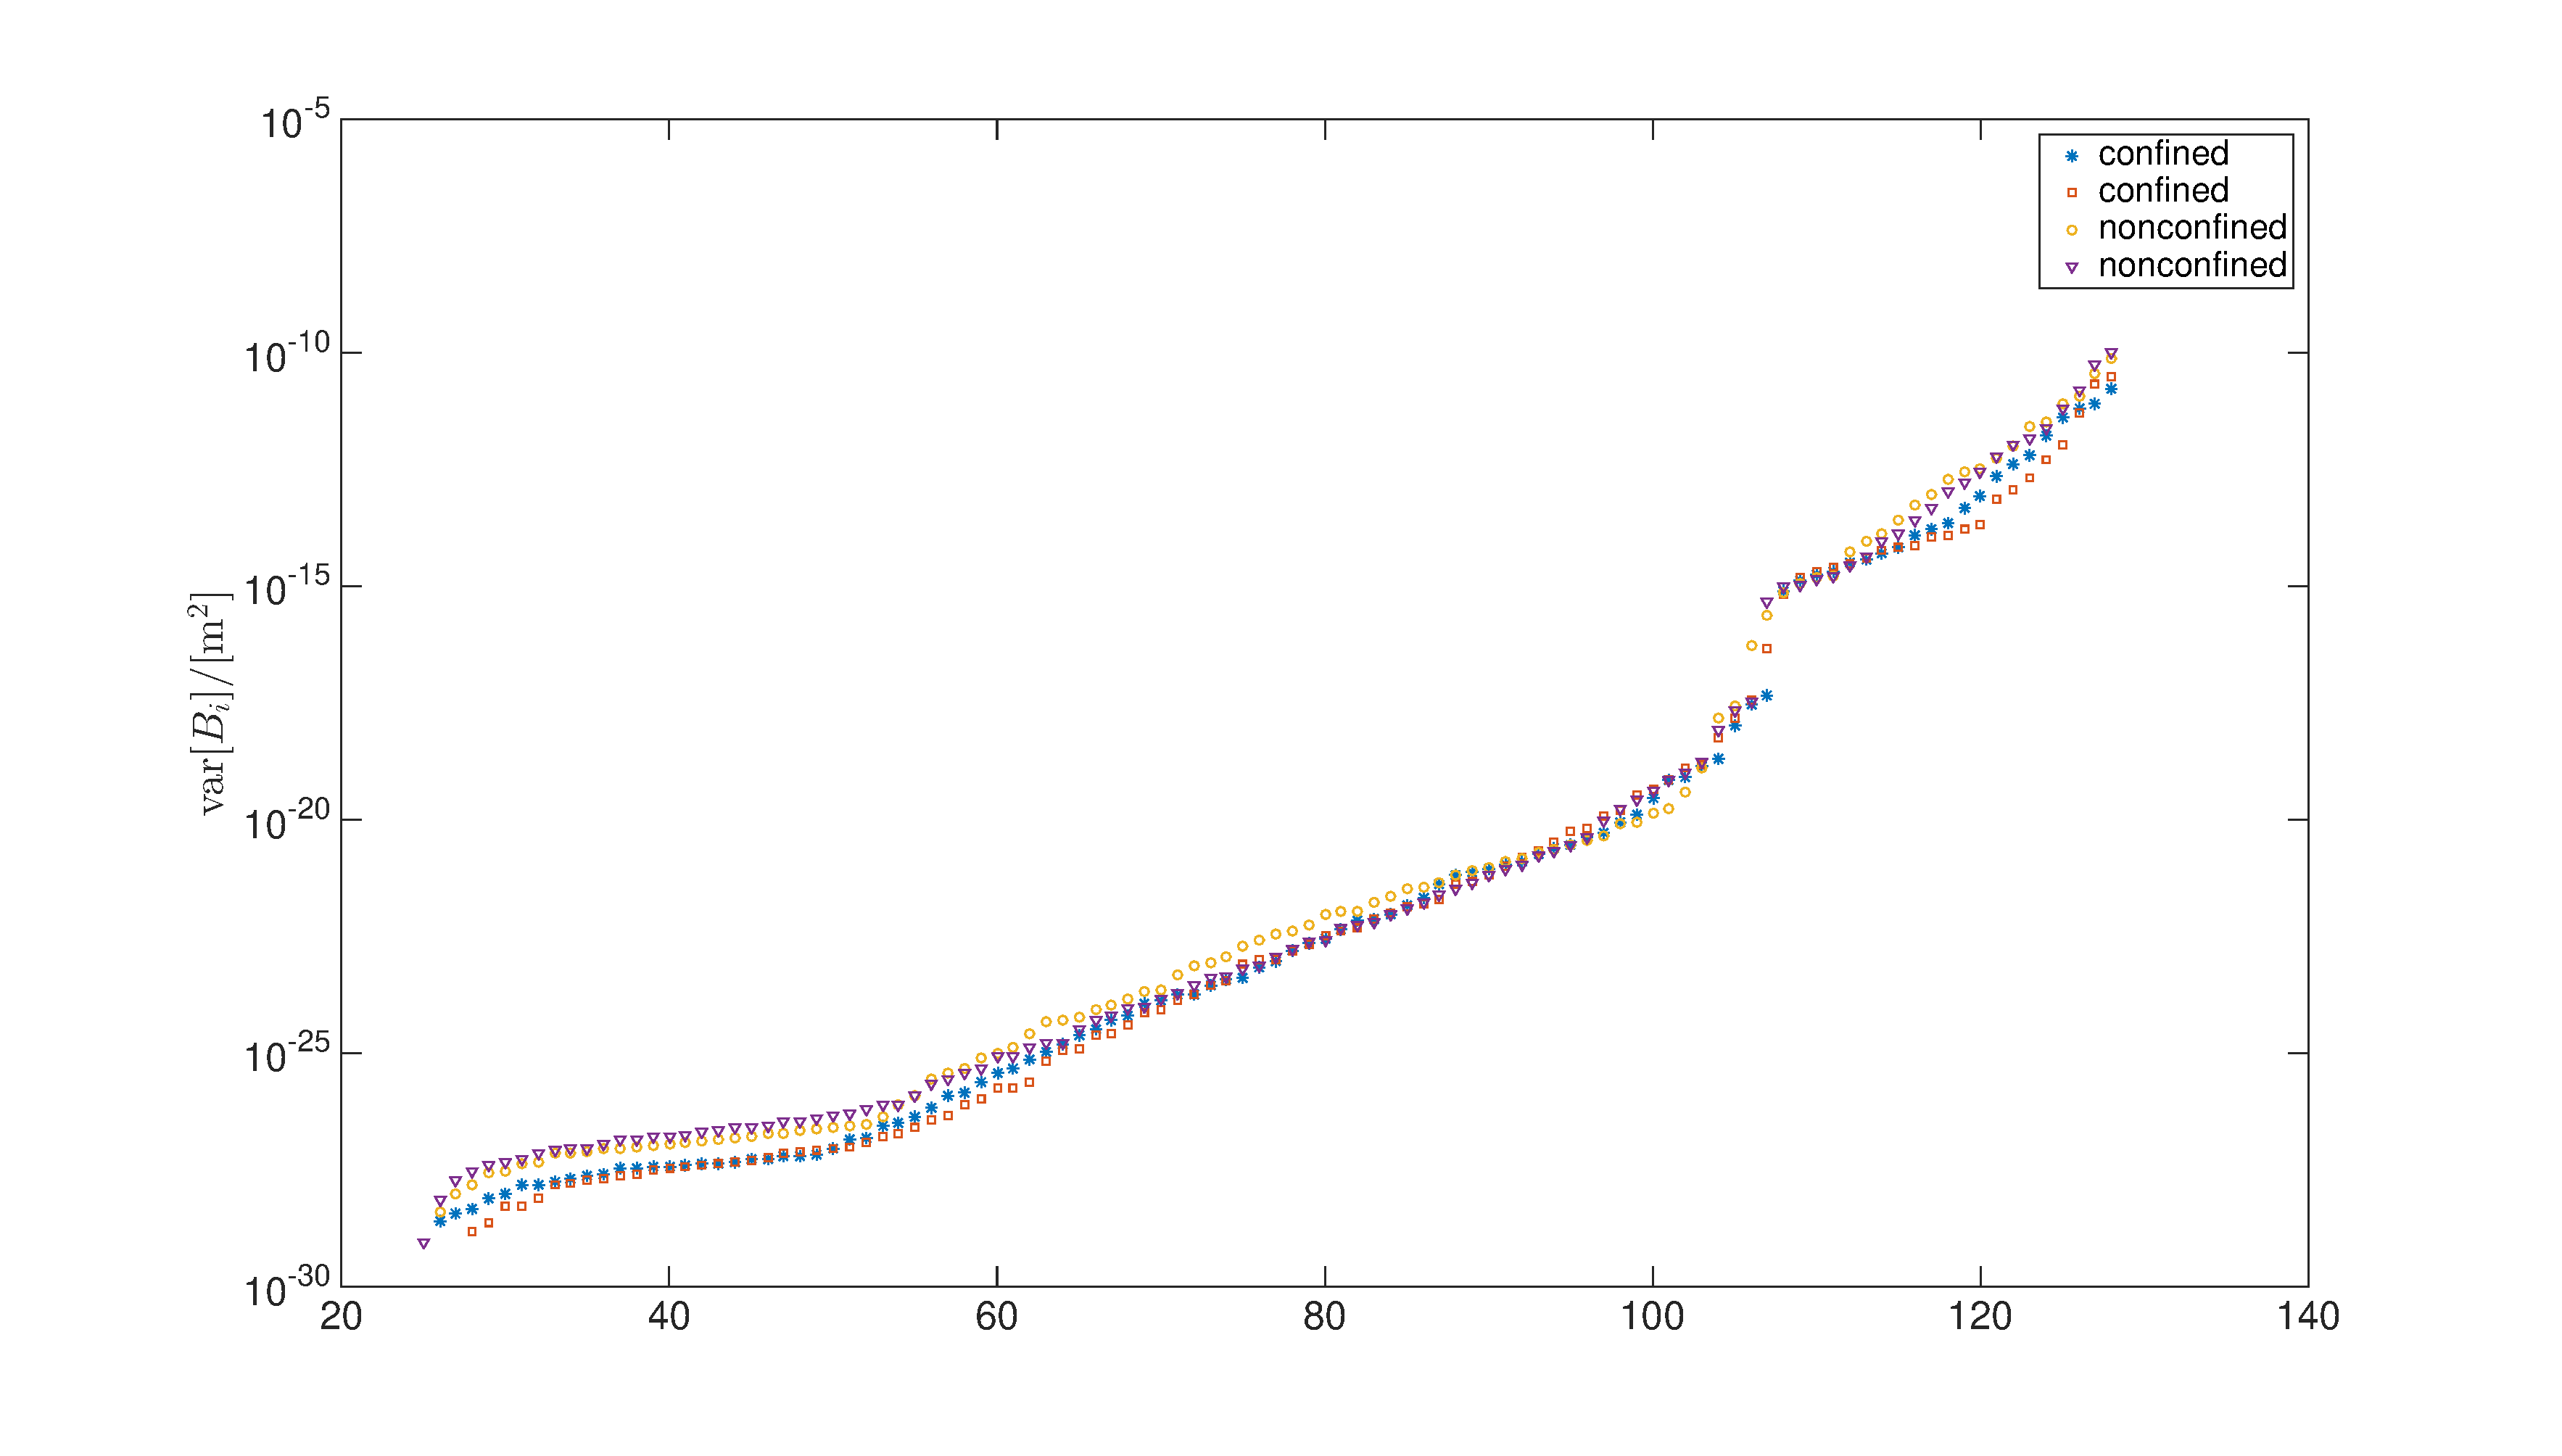
\includegraphics[width=.8\textwidth]{kovegenvarde.eps}
    \caption{Egenvärden till kovariansmatrisen bildad av avståndskomponenter till strängen relativt strängens jämviktsläge för fyra olika strängar. Det största egenvärdent ses vara ungefär $10^{16}$ ggr större än det minsta, vilket påvisar en signifikant skillnad i bidrag till rörelsen från egenmoderna. }
    \label{fig:kovegenvarde}
\end{figure}

\begin{figure}
    \centering
    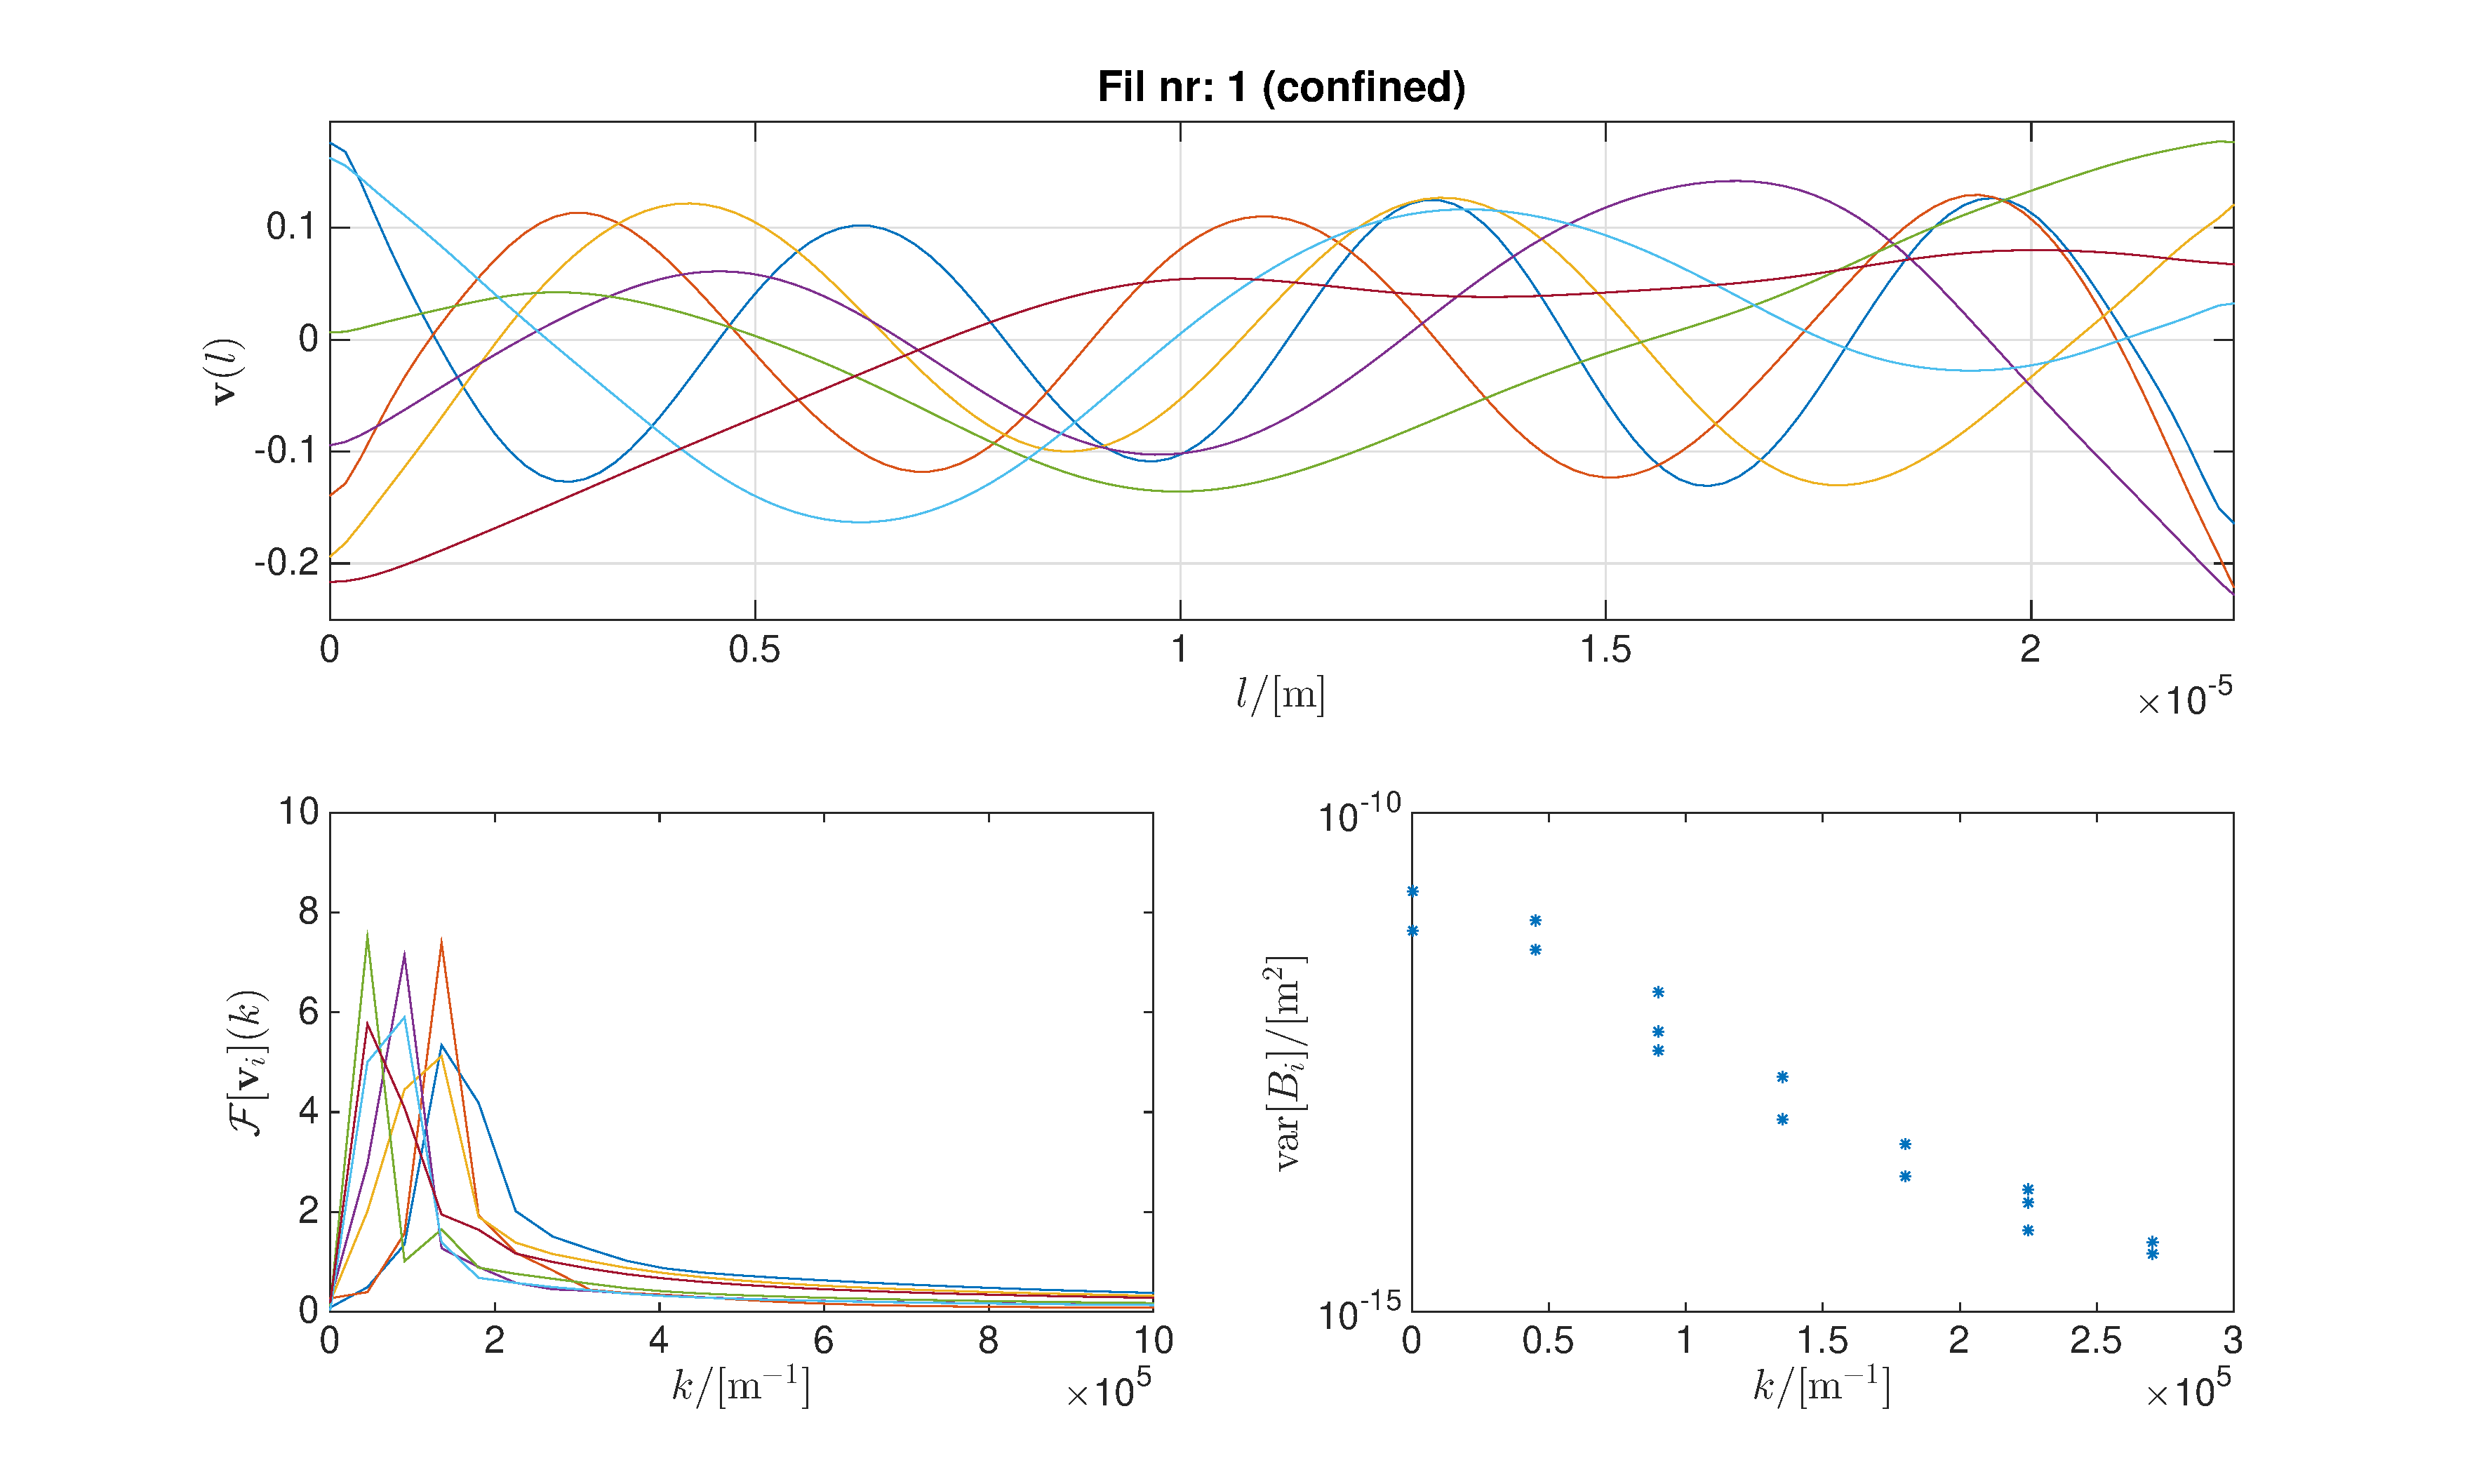
\includegraphics[width=\textwidth]{egenmoder.eps}
    \caption{Caption}
    \label{fig:egenmoder}
\end{figure}

%Resultat som kan tas med

%Motivera att jämviktsläge fanns
%Uppdelningen i egenmoder, olika relaxationstid
%Dispersionsrelation?
%Skillnad mellan confined och unconfined



\section{Diskussion}




%Bara en liten kodsnutt som behövs när man kompilerar lokalt
%%% Local Variables: 
%%% mode: latex
%%% TeX-master: "00main.tex"
%%% End: 


%\chapter{Resultat}

\section{Partikelrörelse i celler}

\subsection{Isometri}

%\subsection{Anisometri} Från givna data kunde en viss tendens till anisometri\todo{anisotropi?} anas då partiklarna tenderade att röra sig längs med vissa riktningar. En minstakvadratanpassning för en rät linje gjordes för att kunna transformera de givna $x$- och $y$-koordinaterna till tangent- och normalkoordinater relativt den anpassade linjen för varje partikel. För dessa nya koordinater beräknades en tidskorrelation vilket visas i \figref{fig:Korr_tn} för både aktiva celler och celler i dvala.

%Tillfällig bild, kan förbättras
%Bör definitivt ändras till eps eller pdf.
%\begin{figure}
%    \centering
%    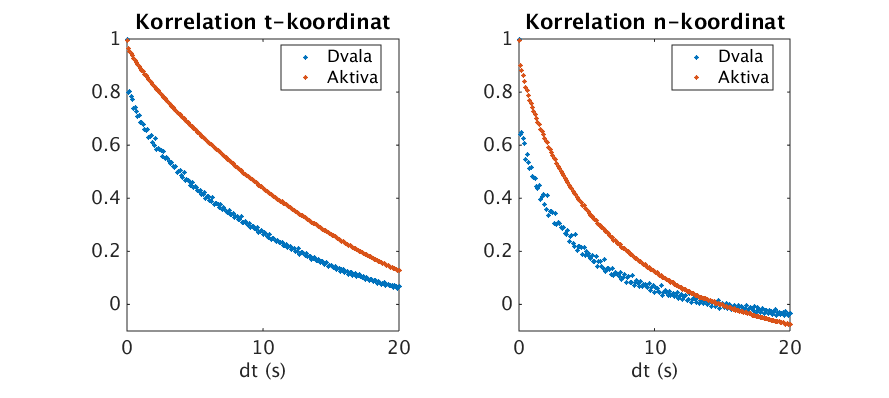
\includegraphics[width=.8\textwidth]{Korrelation_tnkoordinat.png}
%    \caption{Korrelation i tangent- och normal-koordinaterna för aktiva celler och celler i dvala. I båda fall sjunker korrelationen initialt snabbare för cellerna i dvala. Korrelationen tycks även bestå längre i tangentialkoordinaten än normalkoordinaten vilket tyder på att det finns en föredragen väg.}
%    \label{fig:Korr_tn}
%\end{figure}

\subsection{Avvikelse från brownsk rörelse}
%Har vi exempel på avvikelse från teorin kan dessa läggas under seprata underrubriker här

\paragraph{MSD}
Utifrån teorin kring Brownsk rörelse kan vissa förutsägelser göras för partiklar som strikt följer denna typ av rörelse. Bland annat räknades det fram i avsnitt~\ref{sec:brown} att mean square displacement (MSD) för en sådan partikel skulle öka linjärt med tiden, se ekvation \todo{}\eqref{eq:MSD_brown}. Utifrån givna data för arbetet har ett potenssamband kunnat anpassas med en exponent som är skilld från och betydligt lägre än 1. Detta tyder på att partikeln inte utför en ren brownsk rörelse utan genomgår en så kallad subdiffusion, karakteriserat att partikelns MSD beror av tiden via ett potenssamband med exponent mindre än 1 men större än 0.

\begin{figure}
    \centering
    \includegraphics[width=.8\textwidth]{MSD_lilla_delta.png}
    \caption{Från filen MSD.m}
    \label{fig:MSD_ld}
\end{figure}

Vidare finns det minst två sätt att beräkna partiklarnas MSD. För stationära processer, dvs processer som inte explicit beror på när i tiden de inleds, kan man skapa ett medelvärde mellan alla möjliga mätpunkter separerade med givet tidsintervall så som beskrivet i ekvation ...
\todo{Kanske bör vi lägga till ett stycke om hur egenskaperna beräknas utifrån diskret data}
Genom att jämföra resultatet från denna typ av beräkning med att istället bara ta medelvärdet mellan alla partiklars kvadrerade radiella avvikelse från startpunkten vid given tid från start kan man avgöra om processen är stationär.
\todo{Bild för jämförelse mellan lilla och stora delta}
Båda dessa beräkningar har utförts för given data och exponentens värde i sambandet mellan MSD och tid skiljer sig/överensstämmer för lite för att någon tydlig slutsats hurvida processen är stationär eller ej ska kunna dras. \todo{Eller?}

\begin{figure}
    \centering
    \includegraphics[width=.8\textwidth]{MSD_stora_delta.png}
    \caption{Från filen storleksberoende.m}
    \label{fig:MSD_sd}
\end{figure}


%%%%%%%%%%%%%%%%%%%%%%%%%%%%%%Strängar%%%%%%%%%%%%%%%%%%%%%%%%%%%%%%


\section{Strängars rörelse i vätskor}




%Bara en liten kodsnutt som behövs när man kompilerar lokalt
%%% Local Variables: 
%%% mode: latex
%%% TeX-master: "main.tex"
%%% End: 



%\chapter{Diskussion}

\section{Partiklar}

\section{Strängar}


%Bara en liten kodsnutt som behövs när man kompilerar lokalt
%%% Local Variables: 
%%% mode: latex
%%% TeX-master: "main.tex"
%%% End: 


\chapter{Slutsats}

De observerade partiklarna i jästcellerna undergår subdiffusion, det vill säga diffunderar långsammare än en vanlig brownsk rörelse. Därmed ger varken denna modell eller Ornstein-Uhlenbeck-modellen en överensstämmande beskrivning av diffusionstakten. Ornstein-Uhlenbeck-modellen kan dock användas för att beskriva skillnaden i asfärisitet mellan de två cellfaserna \emph{aktiv} och \emph{i dvala}.

Även om fBm och CTRW båda förutsäger subdiffusion kan dessa modeller inte beskriva alla de observerade egenskaperna hos partiklarna. Utifrån anpassningar till partiklarnas MSD, PSD och asfärisitet kan rörelsens Hurstparameter, kopplad till fBm, tas fram. Dessa värden på $H$ överlappar inte vilket tyder på brister i fBm som modell för partikelrörelse i celler. CTRW utgör ingen stationär process något som den observerade processen verkar vara...

%Bara en liten kodsnutt som behövs när man kompilerar lokalt
%%% Local Variables: 
%%% mode: latex
%%% TeX-master: "00main.tex"
%%% End: 




%%%%%%%%%%%%%%%%%%%%%%%%% Källförteckning %%%%%%%%%%%%%%%%%%%%%%%%%
\newpage
\bibliographystyle{ieeetr}
\bibliography{referenser_kandidat}

%%%%%%%%%%%%%%%%%%%%%%%%%%%%% Bilagor %%%%%%%%%%%%%%%%%%%%%%%%%%%%%
\clearpage

\appendix

\chapter{Databehandling}


\section{Datainsamling}
\todo[inline]{Lägg in information i resp. kap.}
Datan som behandlats i denna studie har inte samlats in i samband med denna studie utan tillhandahölls från andra källor. Hur denna data där samlats in och vad den beskriver presenteras mer utförligt nedan.

\subsubsection{Datan för partikelrörelse i celler}
Datan som studerats för partikelrörelser är samma som \cite{Midtveldt_etal2016} använde och utgörs av mätningar av positionen för fluorescerande partiklar i jästceller. Jästcellerna hade genmodifierats till att producera fluorescerande protein som lätt bildar kluster. 
Dessa kluster brukar vara av storleksordning 100--500\,nm, vilket kan jämföras med själva cellernas storlek på omkring 5\,\micro{m}.

Data för ett hundratal partiklar från olika jästceller ingick i mätserien, både för aktiva celler och celler som försatts i dvala med sänkt metabol aktivitet. Mätningen genomfördes med 100 bilder per sekund.


\subsubsection{Datan för strängrörelse i vätska}

Datan som analyserats för strängrörelse i vätska kommer från \todo{Var kommer datan från? Fråga Daniel?}... och består av filmer av aktinfilament som tillåts röra sig i en vätska. Dessa strängar hade en längd kring 10--30\,\micro{m} och befann sig i kanaler av olika bredd. Datan hade redan behandlats något så att strängens läge gav av en uppsättning vita pixlar mot en svart bakgrund.

Mätningar hade utförts på två typer av strängar: fria strängar i breda kanaler och inneslutna strängar i smala skåror. Det fanns två filmer för vardera strängtyp. Alla fyra hade filmats med 10 bilder per sekund. Rörelsen utfördes till största del i två dimensioner då skårornas djup var litet i förhållande till skårornas och filamentens bredd.


\section{Polynomanpassning för strängarna (bättre rubrik?)}
\todo{Förslag: Parametrisering av strängdata}







%Bara en liten kodsnutt som behövs när man kompilerar lokalt
%%% Local Variables: 
%%% mode: latex
%%% TeX-master: "00main.tex"
%%% End: 



\chapter{Beteckningar}
\todo[inline]{Här kan vi ha en lite förklaringslista över vad olika (matematiska) 00beteckningar betyder.}
 \todo{Typ så här?}
\begin{description}[align=left]

\item[fBm] fractional Brownian motion, modell för att beskriva stokastiska processer med inbyggd bestående korrelation mellan stegen.
\item[filament] ...
\item[MSD] Mean squared displacement, sv. medelvärde av kvadrerade avvikelsen.
\item[PSD] Power spectral density, sv. spektrala effekttätheten.
\item[SDE] Stokastisk differentialekvation
\item[WLC] Worm-like chain, en modell för att beskriva polymerers dynamik.

\end{description}



%Bara en liten kodsnutt som behövs när man kompilerar lokalt
%%% Local Variables: 
%%% mode: latex
%%% TeX-master: "00main.tex"
%%% End: 



\end{document}








%% På svenska ska citattecknet vara samma i både början och slut.
%% Använd två apostrofer (två enkelfjongar): ''.

%% Inkludera PDF-dokument
\includepdf[pages={1-}]{filnamn.pdf} %Filnamnet får INTE innehålla 'mellanslag'!

%% Figurer inkluderade som pdf-filer
\begin{figure}\centering
\centerline{ %centrerar även större bilder
\includegraphics[width=1\textwidth]{filnamn.pdf}
}
\caption{\label{fig:} }
\end{figure}

%% Figurer inkluderade med xfigs "Combined PDF/LaTeX"
\begin{figure}\centering
\resizebox{.8\textwidth}{!}{\input{filnamn.pdf_t}}
\caption{\label{fig:} }
\end{figure}

%% Figurer roterade 90 grader
\begin{sidewaysfigure}\centering
\centerline{ %centrerar även större bilder
\includegraphics[width=1\textwidth]{filnamn.pdf}
}
\caption{\label{fig:} }
\end{sidewaysfigure}


%%Om man vill lägga till något i TOC
\stepcounter{section} %Till exempel en 'section'
\addcontentsline{toc}{section}{\Alph{section}\hspace{8 pt}Labblogg} 



%Bara en liten kodsnutt som behövs när man kompilerar lokalt
%%% Local Variables: 
%%% mode: latex
%%% TeX-master: "00main.tex"
%%% End: 